\documentclass{article}

% Language setting
\usepackage[romanian]{babel}

% Set page size and margins
% Replace `letterpaper' with`a4paper' for UK/EU standard size
\usepackage[a4paper,top=2cm,bottom=2cm,left=3cm,right=3cm,marginparwidth=1.75cm]{geometry}

% Useful packages
\usepackage{amsmath}
\usepackage{graphicx}
\usepackage[colorlinks=true, allcolors=blue]{hyperref}
\usepackage{amssymb}
\usepackage{tabto}
\usepackage{multicol}
\usepackage{hyperref}
\usepackage{mdframed}
\usepackage{xcolor}
\usepackage{mathtools}
\usepackage{wrapfig}
\usepackage{listings}

\newcommand\eqdef{\stackrel{\mathclap{\normalfont\mbox{def}}}{=}}
\newcommand\eqnot{\stackrel{\mathclap{\normalfont\mbox{not}}}{=}}

\makeatletter
\renewcommand*\env@matrix[1][c]{\hskip -\arraycolsep
  \let\@ifnextchar\new@ifnextchar
  \array{*\c@MaxMatrixCols #1}}
\makeatother


\hypersetup{
  colorlinks,
  citecolor=violet,
  linkcolor=black,
  urlcolor=blue}

\graphicspath{ {./images/} }

\title{Interpolare}
\author{}
\date{}

\begin{document}
\maketitle

\section{Introducere Interpolare Polinomiala}

\subsection{Notiuni generale}
\tab Fie o functie $f:[a,b]\rightarrow\mathbb{R}.$
Cunoastem valorile functiei intr-un numar redus de puncte $(x_i, f(x_i)), \, i = \overline{0, n}$.
Punctele $x_0, x_1,\dots, x_n$ se numesc \textit{noduri} si formeaza \textit{suportul interpolarii}.

Pornind de la un set discret de puncte, dorim sa construim o functie (polinom) care va trece prin toate aceste puncte.


\begin{minipage}{0.4\textwidth}
    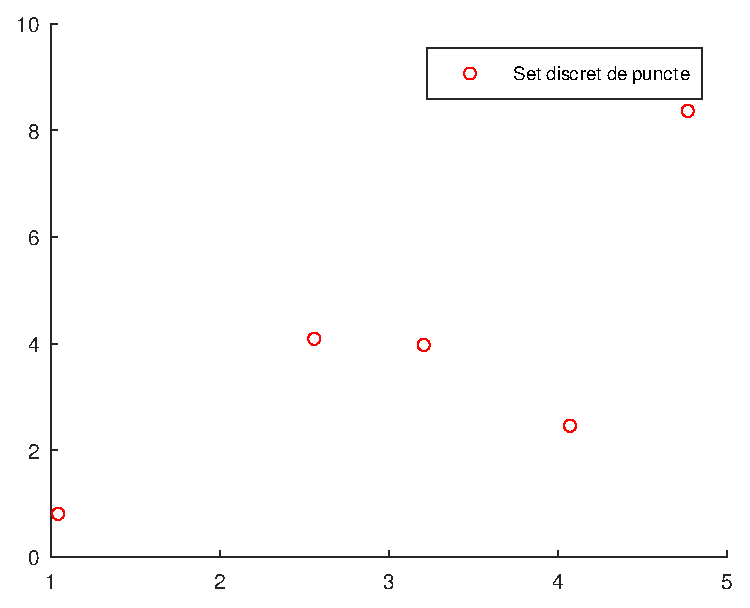
\includegraphics[scale=0.5]{discrete_points_before}
\end{minipage}
{\LARGE$\xrightarrow[Polinomiala]{Interpolare}$}
\begin{minipage}{0.6\textwidth}
    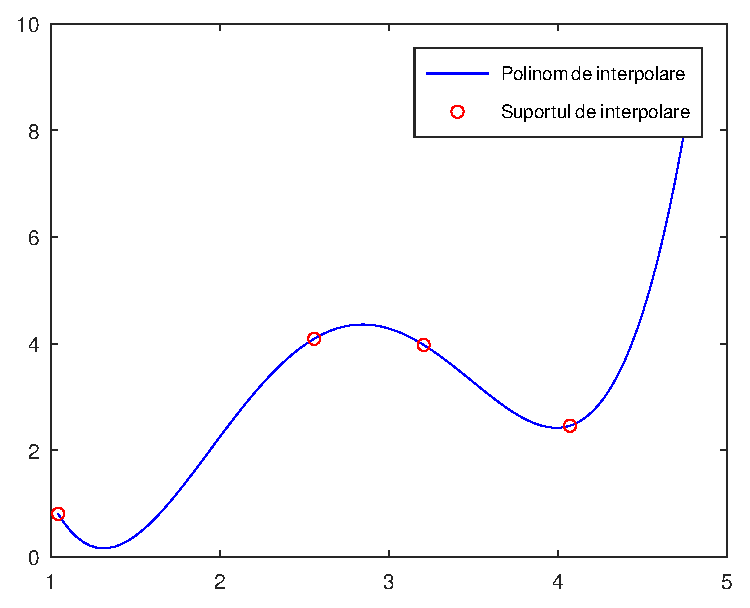
\includegraphics[scale=0.5]{discrete_points_after}
\end{minipage}


\subsection{Motivatie}
\begin{itemize}
    \item In Computer Science se lucreaza in general cu date discrete.
    \item Functii complexe ca forma se pot simplifica, alegand cateva puncte $(x_i, f(x_i))$ si construind pe baza lor niste aproximari cu ajutorul unor polinoame.
    \item Polinoamele sunt usor de evaluat, derivat, integrat, deci interpolarea polinomiala are un avantaj.
\end{itemize}

\subsection{Idee}
\tab Sa presupunem ca se cunoaste valoarea functiei $f(x)$ in $(n+1)$ puncte.
Asadar, suportul interpolarii va arata astfel: $S=[(x_0, f(x_0)), (x_1, f(x_1)),\dots,(x_n, f(x_n))]$.
Deci, $(n+1)$ puncte in care stim valorile functiei pe care dorim sa o aproximam cu un polinom de grad (cel mult) $n$.

La modul general, un polinom de interpolare este o combinatie liniara de functii, de forma: $P_n(x)= a_0\cdot u_0(x) + a_1\cdot u_1(x) + \dots + a_n\cdot u_n(x)$. Functiile $u_0(x), u_1(x), \dots, u_n(x)$ sunt liniar independente si formeaza \textit{baza interpolarii}. $a_0, a_1, \dots, a_n$ reprezinta coeficientii care trebuie determinati.

\subsection{Conditii de interpolare}
\tab Polinomul de interpolare construit $P_n(x)$ trebuie sa coincida cu functia initiala pe suportul interpolarii. Matematic, afirmatia devine: $P_n(x_i) = f(x_i), \forall \, i = \overline{0, n}$.

\subsection{Teorema Weierstrass}
\tab Fie o functie continua $f:[a,b]\rightarrow\mathbb{R}$ si $\epsilon > 0 \, (toleranta)$. Atunci $\exists\; P(x) \in \mathbb{R}^{n}$, a.\^{i}. \framebox{$|f(x)-P(x)| < \epsilon$}, $\forall \, x \in [a, b]$.

Asadar, teorema ne asigura ca pentru orice functie continua pe un interval $[a,b]$, exista un polinom cu care putem aproxima functia.\\

\subsection{Tipuri de interpolari abordate}
\begin{multicols}{2}
    \begin{itemize}
    
        \item Interpolare \textit {polinomiala} de tip:
        \begin{itemize}
            \item \framebox{\textbf{\hyperref[sec:vandermonde]{Vandermonde}}}
            \item \framebox{\textbf{\hyperref[sec:lagrange]{Lagrange}}}
            \item \framebox{\textbf{\hyperref[sec:newton]{Newton (Diferente Divizate)}}}
        \end{itemize}
        
        \item Interpolare folosind functii \textit {spline}:
        \begin{itemize}
            \item \framebox{\textbf{\hyperref[sec:liniare]{Liniare}}}
            \item \framebox{\textbf{\hyperref[sec:spline_c1]{Cubice de clasa $C^1$}}}
            \item \framebox{\textbf{\hyperref[sec:spline_c2]{Cubice de clasa $C^2$}}}
        \end{itemize}
    
    \end{itemize}
\end{multicols}

\subsection{Aplicatii din viata reala care folosesc interpolarea}

\begin{itemize}

    \item \textbf {Image scaling}
    
    \tabto{0.5cm} Exemplu: Daca avem o \textit{imagine} (cu un singur canal de culoare) de dimensiune $2\times2$ pixeli si dorim sa o marim de 2 ori, ne putem folosi de tehnica de interpolare.
    
    \;\;\;\;\;\;\;\;
    \begin{minipage}{0.225\textwidth}
        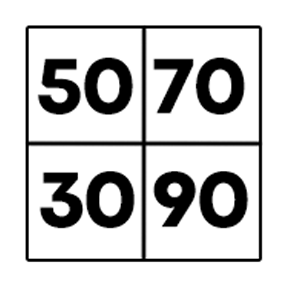
\includegraphics[scale=0.75]{img_scale_before}
    \end{minipage}
    {\LARGE$\xrightarrow[Biliniara]{Interpolare}$}\;\;
    \begin{minipage}{0.775\textwidth}
        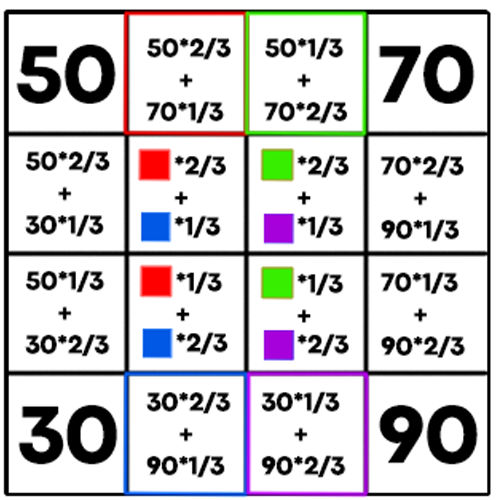
\includegraphics[scale=1.5]{img_scale_after_color}
    \end{minipage}

     
    Pentru acest exemplu s-a aplicat o interpolare biliniara
    \framebox[0.3cm][r]{\footnotemark} cu coeficientii $\frac{1}{3}$ si $\frac{2}{3}$.
    \footnotetext{\framebox[8cm]{\url{https://en.wikipedia.org/wiki/Bilinear_interpolation}}}

    \item \textbf {Filling missing values}
    
    \tabto{0.5cm} Exemplu: O firma isi monitorizeaza vanzarile zilnic, timp de o saptamana, insa in ziua a 5-a a omis masuratoarea. Ce cantitate de produse (aproximativ) a vandut in ziua a 5-a? \\
    
    \begin{minipage}{0.5\textwidth}
        \tabto{0.5cm} Sa presupunem ca graficul vanzarilor\\
        arata astfel:\\\\\\\\
        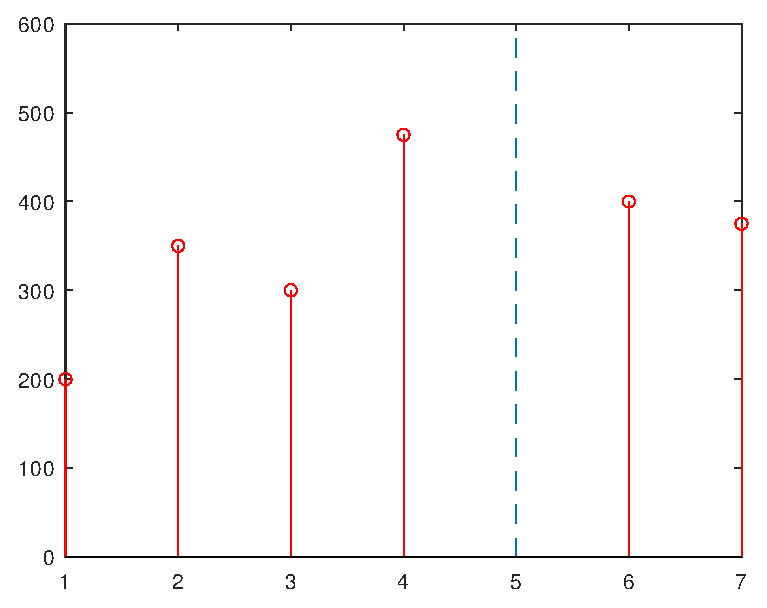
\includegraphics[width=0.8\textwidth]{sales_before}
    \end{minipage}
    \begin{minipage}{0.5\textwidth}
        \tabto{0.5cm} Folosind o interpolare polinomiala, gasim un polinom care trece prin cele 6 puncte cunoscute si astfel putem aproxima cantitatea de produse vanduta in ziua a 5-a.\\\\
        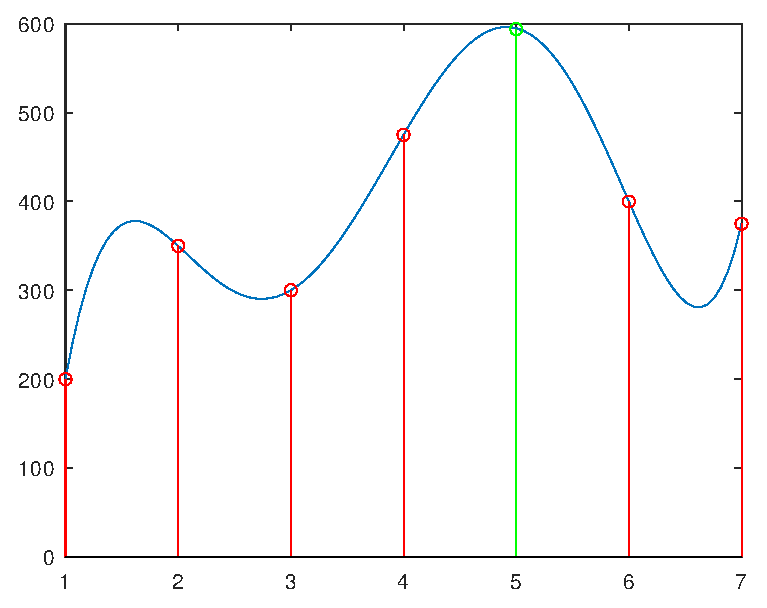
\includegraphics[width=0.8\textwidth]{sales_after}
    \end{minipage}
    
\end{itemize}

\subsection{Pregatirea terenului}
\tab Inainte de a discuta despre fiecare tip de interpolare, prezentam cadrul discutiei: 

\begin{itemize}

    \item Pornim de la o  functie continua $f:[a,b]\rightarrow\mathbb{R}$ careia ii cunoastem valorile in $(n+1)$ puncte.
    
    \item Asadar, suportul interpolarii va fi de forma: $S=[(x_0, f(x_0)), (x_1, f(x_1)),\dots, (x_n, f(x_n))]$.
    
    \item Dorim sa gasim un polinom de grad (cel mult) $n$ care sa aproximeze functia $f(x)$.
    
\end{itemize}


\section{Interpolare Vandermonde}
\label{sec:vandermonde}

\subsection{Baza de interpolare}

\tab Interpolarea Vandermonde foloseste ca baza de interpolare, baza polinoamelor: $\{1, x, x^2,\dots, x^n\}$.\vspace{0.15cm}
\tabto{0.5cm} Deci, polinomul de interpolare Vandermonde arata astfel:
\framebox{$P_n(x)= a_0 \cdot 1 + a_1 \cdot x + a_2 \cdot x^2 + \dots + a_n \cdot x^n$}\vspace{0.05cm}

Pentru a determina coeficientii $a_0, a_1, \dots, a_n$, punem conditiile de interpolare: 
\framebox{$P_n(x_i) = f(x_i), \forall \, i = \overline{0, n}$}

\begin{equation*}
    \begin{cases}
      Pentru\;\; i=0: P_n(x_0) = f(x_0) \iff a_0 + a_1\cdot x_0 + a_2\cdot x_0^2 + \dots + a_n\cdot x_0^n = f(x_0)\\
      
      Pentru\;\; i=1: P_n(x_1) = f(x_1) \iff a_0 + a_1\cdot x_1 + a_2\cdot x_1^2 + \dots + a_n\cdot x_1^n = f(x_1)\\
      
      \;\dots\\
      
      Pentru\;\; i=n: P_n(x_n) = f(x_n) \iff a_0 + a_1\cdot x_n + a_2\cdot x_n^2 + \dots + a_n\cdot x_n^n = f(x_n)
    \end{cases}
\end{equation*}

Sistemul de mai sus poate fi scris sub forma matriceala, astfel: 

\newenvironment{sbmatrix}[1]
 {\def\mysubscript{#1}\mathop\bgroup\begin{bmatrix}}
 {\end{bmatrix}\egroup_{\textstyle\mathstrut\mysubscript}}

\[
\begin{sbmatrix}{A}
    1 & x_0 & x_0^2 & \dots & x_0^n \\
    1 & x_1 & x_1^2 & \dots & x_1^n \\
    \vdots & \vdots & \vdots & \ddots & \vdots \\
    1 & x_n & x_n^2 & \dots & x_n^n \\
\end{sbmatrix}
\cdot
\begin{sbmatrix}{x}
    a_0 \\
    a_1 \\
    \vdots \\
    a_n \\
\end{sbmatrix}
=
\begin{sbmatrix}{b}
    f(x_0) \\
    f(x_1) \\
    \vdots \\
    f(x_n) \\
\end{sbmatrix}
\]


Asadar, avem de rezolvat un sistem de forma $A\cdot x = b$.

Matricea $A$ (de tip Vandermonde) este nesingulara \framebox[0.3cm][r]{\footnotemark},
\footnotetext{\framebox[13.5cm]{\url{https://math.stackexchange.com/questions/426932/why-are-vandermonde-matrices-invertible}}}
deci sistemul are solutie unica, ceea ce conduce la uniticitatea polinomul de interpolare
\framebox[0.3cm][r]{\footnotemark}.
\footnotetext{\framebox[15cm]{\url{https://en.wikipedia.org/wiki/Polynomial_interpolation\#Uniqueness_of_the_interpolating_polynomial}}}


\subsection{Exemplu numeric}
\tab Sa consideram cunoscute urmatoarele puncte din plan: $\{(1,1), (2,8), (3,27)\}$.

\begin{tabular}{c | c | c | c}
    $x$ & 1 & 2 & 3 \\
    \hline
    $f(x)$ & 1 & 8 & 27 \\
\end{tabular}
$\Rightarrow$ Avem urmatoarele noduri: $x_0=1;\; x_1=2;\; x_2=3$.

Suportul interpolarii este $S=[(1,1), (2,8), (3,27)]$.

Asadar, avand 3 puncte in suportul interpolarii, cautam un polinom de interpolare de grad 2.

Deci, polinomul cautat are forma: $P_2(x) = a_0 + a_1\cdot x + a_2 \cdot x^2$.

Punand conditiile de interpolare, vom avea de rezolvat urmatorul SEL (sistem de ecuatii liniare):

\[
\begin{bmatrix}
    1 & x_0 & x_0^2 \\
    1 & x_1 & x_1^2 \\
    1 & x_2 & x_2^2 \\
\end{bmatrix}
\cdot
\begin{bmatrix}
    a_0 \\
    a_1 \\
    a_2 \\
\end{bmatrix}
=
\begin{bmatrix}
    f(x_0) \\
    f(x_1) \\
    f(x_2) \\
\end{bmatrix}
\iff
\begin{bmatrix}
    1 & 1 & 1^2 \\
    1 & 2 & 2^2 \\
    1 & 3 & 3^2 \\
\end{bmatrix}
\cdot
\begin{bmatrix}
    a_0 \\
    a_1 \\
    a_2 \\
\end{bmatrix}
=
\begin{bmatrix}
    1 \\
    8 \\
    27 \\
\end{bmatrix}
\xRightarrow[\text{}]{\text{(\dots)}}
\framebox{
$\begin{cases}
  a_0 = 6 \\
  a_1 = -11 \\
  a_2 = 6 \\
\end{cases}$}
\]

$\Rightarrow P_2(x) = 6 - 11 \cdot x + 6 \cdot x^2 \; \Rightarrow \framebox{$P_2(x) = 6 \cdot x^2 - 11 \cdot x + 6$}$\\

\begin{minipage}{0.4\textwidth}
    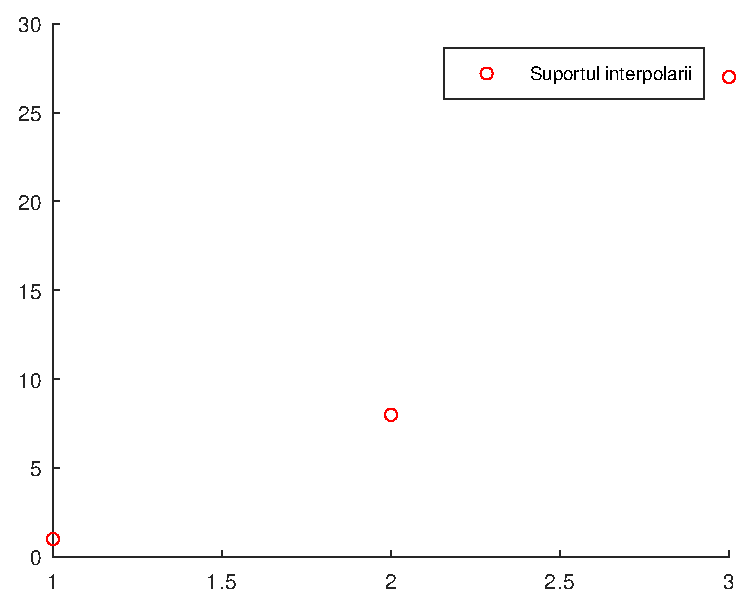
\includegraphics[width=1\textwidth]{scatter_ex}
\end{minipage}
{\LARGE$\xrightarrow[Vandermonde]{Interpolare}$}\;\;
\begin{minipage}{0.6\textwidth}
    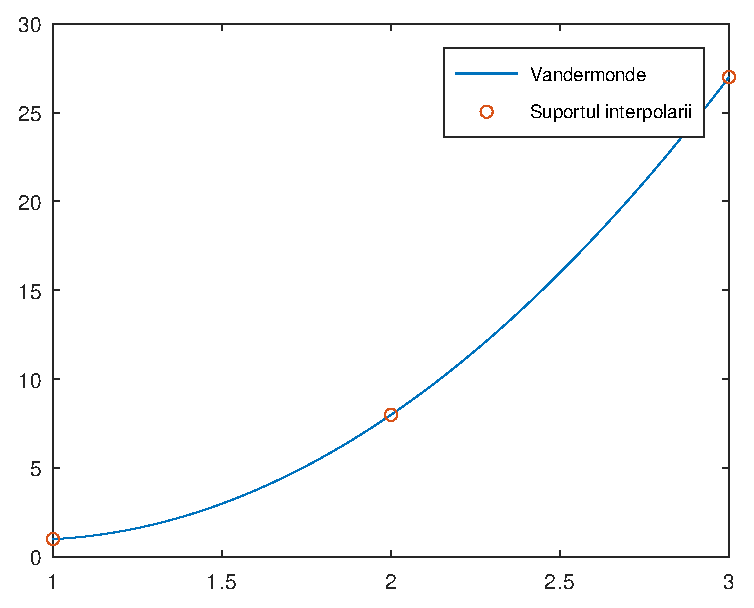
\includegraphics[width=0.68\textwidth]{vandermonde_ex}
\end{minipage}\\\\


\subsection{Concluzii}
\tab Asadar, folosind baza de interpolare Vandermonde $\{1, x, x^2, \dots, x^n\}$, obtinem sistemul:

\[
\begin{sbmatrix}{A}
    1 & x_0 & x_0^2 & \dots & x_0^n \\
    1 & x_1 & x_1^2 & \dots & x_1^n \\
    \vdots & \vdots & \vdots & \ddots & \vdots \\
    1 & x_n & x_n^2 & \dots & x_n^n \\
\end{sbmatrix}
\cdot
\begin{sbmatrix}{x}
    a_0 \\
    a_1 \\
    \vdots \\
    a_n \\
\end{sbmatrix}
=
\begin{sbmatrix}{b}
    f(x_0) \\
    f(x_1) \\
    \vdots \\
    f(x_n) \\
\end{sbmatrix}
\]

$\ominus$ Matricea Vandermonde $A$ este o matrice rau conditionata.\\
    
$\ominus$ Pentru un numar mare de puncte ($n$ mare), matricea $A$ devine matrice plina mare, ceea ce conduce la numar de conditionare mare.\\

$\ominus$ Numarul de conditionare mare implica instabilitate numerica.\\

In concluzie, interpolarea Vandermonde nu este utilizata in practica $\rightarrow$ Cautam alte baze de interpolare.\\


\section{Interpolare Lagrange}
\label{sec:lagrange}

\subsection{Baza de interpolare}
\tab Interpolarea Lagrange foloseste $(n+1)$ polinoame $L_k(x),\; i = \overline{0, n}$.  $L_k(x)$ sunt polinoame de grad (cel mult) $n$ si se numesc \textit{multiplicatori Lagrange}.

Matematic, multiplicatorul Lagrange se defineste astfel: \framebox{$L_k(x) = \prod\limits_{\substack{i=0 \\ i\neq k}}^{n} \frac{x-x_i}{x_k-x_i},\; k = \overline{0, n}$}

Deci, polinomul de interpolare Lagrange se poate scrie:\: \framebox{$P_n(x)= \sum\limits_{k=0}^{n} L_k(x) \cdot f(x_k)$}\\

Pentru a intelege mai bine, particularizam problema la 2 puncte in suportul interpolarii ($n = 1$): $\Rightarrow$ $S=[(x_0, f(x_0),(x_1, f(x_1)]$.

Astfel, multiplicatorii Lagrange vor fi: $L_0(x) = \frac{x-x_1}{x_0-x_1}$ si $L_1(x) = \frac{x-x_0}{x_1-x_0}$.

Tinand cont de forma generala a polinomului de interpolare Lagrange, putem particulariza pe exemplu nostru: $P_1(x) = L_0(x) \cdot f(x_0) + L_1(x) \cdot f(x_1) \iff P_1(x) = \frac{x-x_1}{x_0-x_1} \cdot f(x_0) + \frac{x-x_0}{x_1-x_0} \cdot f(x_1)$.\\

Observatie: Multiplicatorul Lagrange la forma generala $L_k(x_i)$ poate fi privit ca un intrerupator, deoarece pentru $i = k$, acesta este $0$ (\textbf{OFF}), iar pentru $i \neq k$ este $1$ (\textbf{ON}).

De exemplu:
\begin{itemize}
    \item $L_0(x_i) \; \eqdef \; \prod\limits_{\substack{i=0 \\ i\neq 0}}^{n} \frac{x-x_i}{x_0-x_i} \iff L_0(x_i) = \frac{x-x_1}{x_0-x_1} \cdot \frac{x-x_2}{x_0-x_2} \dots \frac{x-x_n}{x_0-x_n} \iff L_0(x_i) =
    \begin{cases}
      0,\; i = 0\\
      1,\; i \neq 0\\
    \end{cases}$
    
    \item Procedand analog, obtinem generalizarea: \framebox{$L_k(x_i) =
    \begin{cases}
      0,\; i = k\\
      1,\; i \neq k\\
    \end{cases}$}
    \textbf{(*)}
\end{itemize}


Un alt aspect important este respectarea conditiilor de interpolare. Este usor de observat faptul ca polinomul de interpolare Lagrange respecta conditiile de interpolare:

Stim ca, la modul general, polinomul de interpolare Lagrange este: $P_n(x) \; \eqdef \; \sum\limits_{k=0}^{n} L_k(x) \cdot f(x_k)$

\begin{itemize}
    \item Pentru $x = x_0$: $P_n(x_0) = L_0(x_0) \cdot f(x_0) + L_1(x_0) \cdot f(x_1) + \dots + L_n(x_0) \cdot f(x_n)$\\
    Conform \textbf{(*)}:
    $\mathbf{L_0(x_0) = 1}$; $L_1(x_0) = 0$; $L_2(x_0) = 0$; $L_3(x_0) = 0; \dots$; $L_n(x_0) = 0$\\
    $\Longrightarrow$ \framebox{$P_n(x_0) = f(x_0)$}
    
    \item Pentru $x = x_1$: $P_n(x_1) = L_0(x_1) \cdot f(x_0) + L_1(x_1) \cdot f(x_1) + \dots + L_n(x_1) \cdot f(x_n)$\\
    Conform \textbf{(*)}:
    $L_0(x_1) = 0$; $\mathbf{L_1(x_1) = 1}$; $L_2(x_1) = 0$; $L_3(x_1) = 0$; \dots; $L_n(x_1) = 0$\\
    $\Longrightarrow$ \framebox{$P_n(x_1) = f(x_1)$}
    
    \item \dots
    
    \item Pentru $x = x_n$: $P_n(x_n) = L_0(x_n) \cdot f(x_0) + L_1(x_n) \cdot f(x_1) + \dots + L_n(x_n) \cdot f(x_n)$\\
    Conform \textbf{(*)}:
    $L_0(x_n) = 0$; $L_1(x_n) = 0$; $L_2(x_n) = 0$; $L_3(x_n) = 0$; \dots; $\mathbf{L_n(x_n) = 1}$\\
    $\Longrightarrow$ \framebox{$P_n(x_n) = f(x_n)$}
\end{itemize}

Asadar, \framebox{$P_n(x_i) = f(x_i), \forall i = \overline{0, n}$} $\Longrightarrow$ Conditiile de interpolare se verifica.


\subsection{Exemplu numeric}
\tab Sa consideram cunoscute urmatoarele puncte din plan: $\{(1,1), (2,8), (3,27)\}$.

\begin{tabular}{c | c | c | c}
    $x$ & 1 & 2 & 3 \\
    \hline
    $f(x)$ & 1 & 8 & 27 \\
\end{tabular}
$\Rightarrow$ Avem urmatoarele noduri: $x_0=1;\; x_1=2;\; x_2=3$.

Suportul interpolarii este $S=[(1,1), (2,8), (3,27)]$.

Asadar, avand 3 puncte in suportul interpolarii, cautam un polinom de interpolare de grad 2.\\

Tinand cont de forma generala a polinomului de interpolare Lagrange, putem particulariza pe exemplul nostru, astfel:
\framebox{$P_2(x) = L_0(x) \cdot f(x_0) + L_1(x) \cdot f(x_1) + L_2(x) \cdot f(x_2)$}


Scriem desfasurat fiecare multiplicator Lagrange, tinand cont de valorile efective ale nodurilor:

\begin{itemize}
    \item $L_0(x) \; \eqdef \; \frac{(x-x_1) \cdot (x-x_2)}{(x_0-x_1) \cdot (x_0-x_2)} = \frac{(x-2) \cdot (x-3)}{(1-2) \cdot (1-3)} = \frac{(x-2) \cdot (x-3)}{2}$
    
    \item $L_1(x) \; \eqdef \; \frac{(x-x_0) \cdot (x-x_2)}{(x_1-x_0) \cdot (x_1-x_2)} = \frac{(x-1) \cdot (x-3)}{(2-1) \cdot (2-3)} = -(x-1) \cdot (x-3)$
    
    \item $L_2(x) \; \eqdef \; \frac{(x-x_0) \cdot (x-x_1)}{(x_2-x_0) \cdot (x_2-x_1)} = \frac{(x-1) \cdot (x-2)}{(3-1) \cdot (3-2)} = \frac{(x-1) \cdot (x-2)}{2}$
\end{itemize}

$\implies P_2(x) = 1 \cdot \frac{(x-2) \cdot (x-3)}{2} + 8 \cdot -(x-1) \cdot (x-3) + 27 \cdot \frac{(x-1) \cdot (x-2)}{2} \implies$\\

$\implies\framebox{$P_2(x) = \frac{1}{2} \cdot (x-2)(x-3) - 8 \cdot (x-1)(x-3) + \frac{27}{2} \cdot (x-1)(x-2)$}$\\


\begin{minipage}{0.4\textwidth}
    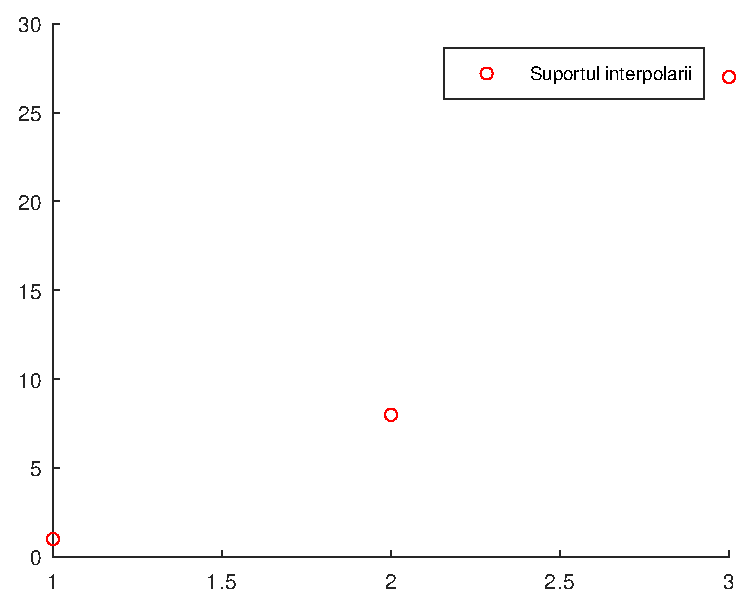
\includegraphics[width=1\textwidth]{scatter_ex}
\end{minipage}
{\LARGE$\xrightarrow[Lagrange]{Interpolare}$}\;\;
\begin{minipage}{0.6\textwidth}
    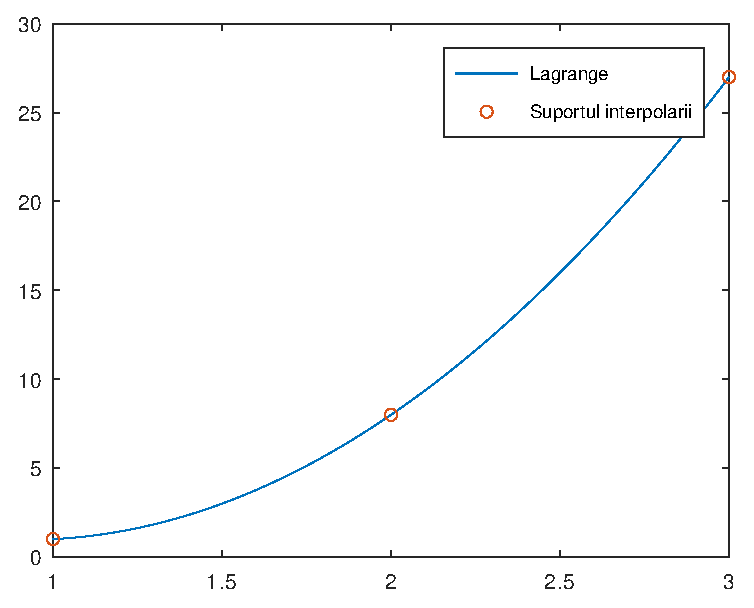
\includegraphics[width=0.68\textwidth]{lagrange_ex}
\end{minipage}\\


\subsection{Fenomenul Runge}
\tab \textit{Functia Runge}\framebox[0.3cm][r]{\footnotemark} se defineste astfel: $f:[-1,1]\rightarrow\mathbb{R},\; f(x) = \frac{1}{1 + 25 \cdot x^2}$
\begin{center}
    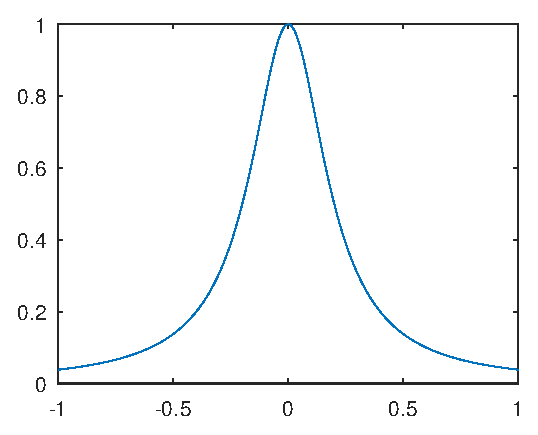
\includegraphics[width=0.2\textwidth]{runge_function}
\end{center}

\footnotetext{\framebox[7.75cm]{\url{https://en.wikipedia.org/wiki/Runge\%27s_phenomenon}}}

Aplicand tehnica de interpolare Lagrange si considerand pe rand $5$, $10$, $15$ si apoi $20$ puncte (echidistante) in suportul de interpolare, obtinem urmatoarele polinoame de interpolare:

\begin{center}
    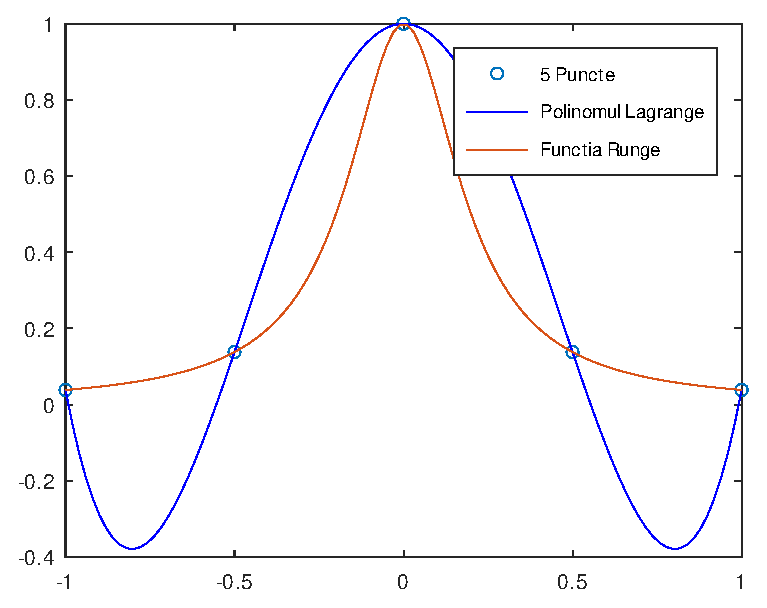
\includegraphics[scale=0.5]{runge_5points}
    \hspace{0.5cm}\vspace{0.25cm}
    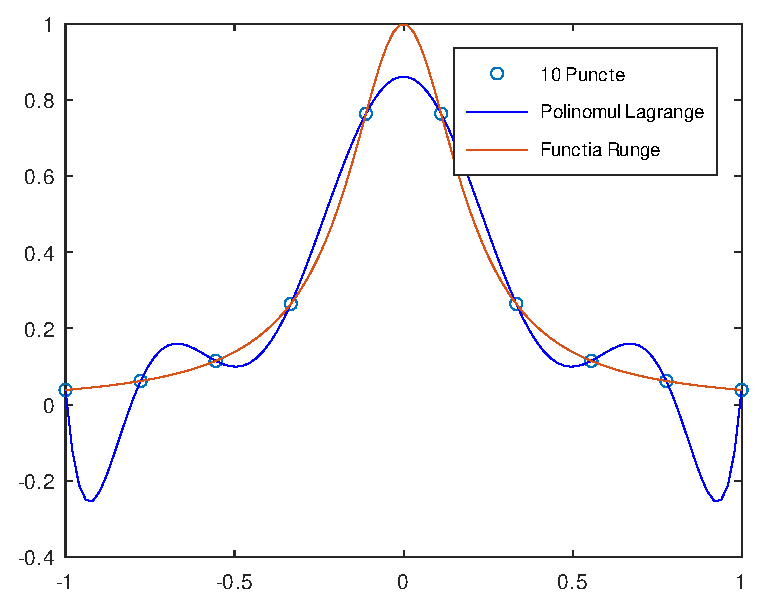
\includegraphics[scale=0.5]{runge_10points}
    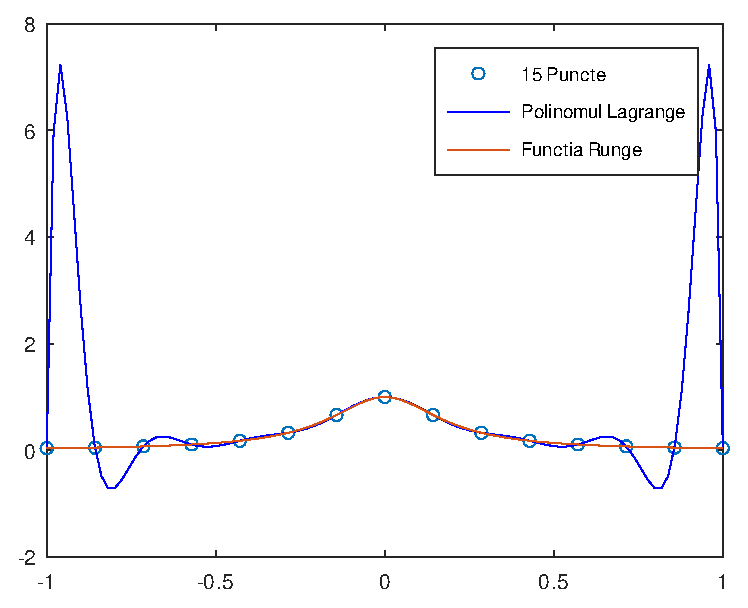
\includegraphics[scale=0.5]{runge_15points}
    \hspace{0.5cm}\vspace{0.25cm}
    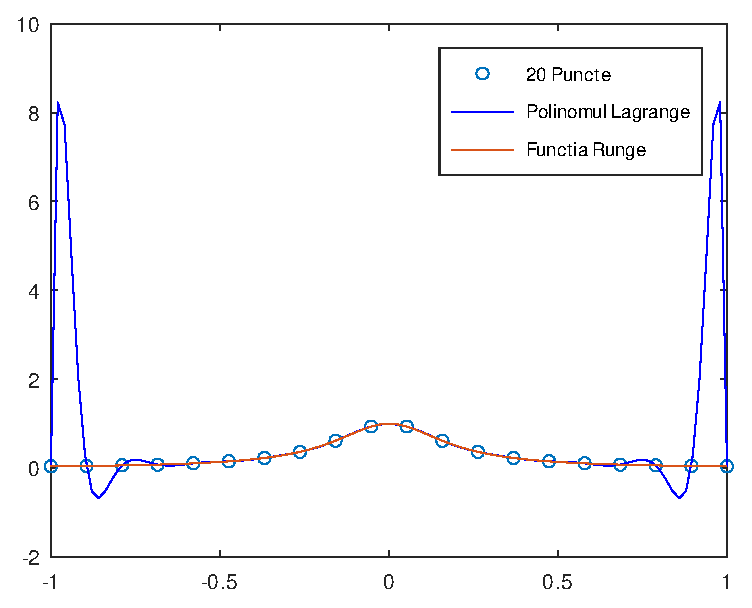
\includegraphics[scale=0.5]{runge_20points}
\end{center}

Asadar, cu cat numarul de puncte din suportul interpolarii creste ($n \uparrow$), gradul polinomului de interpolare creste si polinomul oscileaza in capete, adica eroarea de interpolare creste. Acest fenomen este cunoscut sub denumirea de \textit{fenomen Runge}. \framebox{\href{https://demonstrations.wolfram.com/RungesPhenomenon/}{Animatie}} \\

Observatie: Daca punctele din suportul interpolarii ar fi fost alese la intamplare (sa nu fie echidistante), polinomul ar fi oscilat si mai mult in capete.\\

\noindent\begin{minipage}{0.45\textwidth}
    \tabto{0.5cm} O solutie de atenuare a oscilatiilor este schimbarea modului de distribuire a nodurilor din suportul de interpolare. Un exemplu clasic este setul de noduri Chebyshev \framebox[0.3cm][r]{\footnotemark} pentru care eroarea maximala de aproximare a functiei Runge se diminueaza odata cu cresterea gradului polinomului de interpolare.
\end{minipage}
\hfill
\begin{minipage}{0.5\textwidth}
    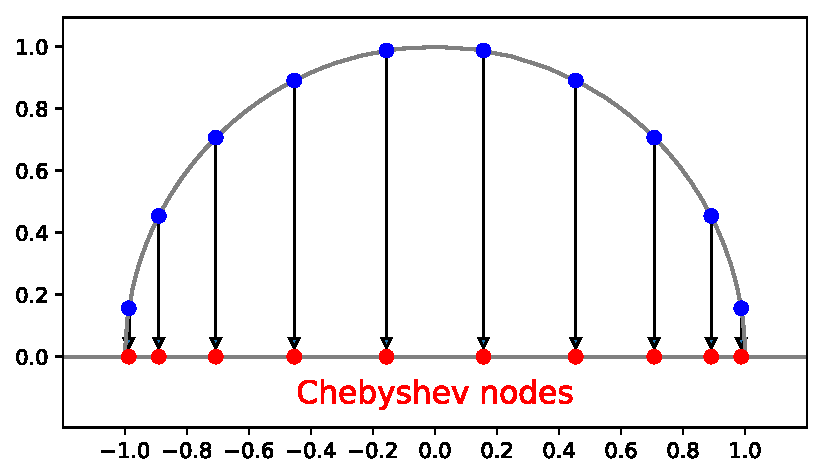
\includegraphics[scale=0.5]{chebyshev_nodes}
\end{minipage}\\

\footnotetext{\framebox[7cm]{\url{https://en.wikipedia.org/wiki/Chebyshev_nodes}}}

Discutia in amanunt a atenuarii oscilatiilor polinomului de interpolare Lagrange nu este de interes in acest moment.\framebox[0.3cm][r]{\footnotemark}

\footnotetext{\framebox[11.75cm]{\url{https://en.wikipedia.org/wiki/Runge\%27s_phenomenon\#Mitigations_to_the_problem}}}


\subsection{Concluzii}
\tab
$\oplus$ Metoda Lagrange este mai robusta decat Vandermonde.\\

$\oplus$ Folosita in cadrul academic.\\

$\ominus$ Instabila numeric pentru calculul polinomului.\\

$\ominus$ Polinomul de interpolare oscileaza in capete.\\


\section{Interpolare Newton (Diferente Divizate)}
\label{sec:newton}

\subsection{Baza de interpolare}

\begin{itemize}
    \item La interpolarea Newton, scriem polinomul de interpolare in functie de \framebox{$(x-x_i)$} in loc de $x$.
    
    \item \textbf{Deducerea formulelor:}
    \begin{itemize}
        \item Interpolare polinomiala \textbf{liniara} $\rightarrow$ Suportul de interpolare este format din 2 puncte: $S=[(x_0, f(x_0)), (x_1, f(x_1))]$.\\
        Polinomul de interpolare va avea urmatoarea forma:
        
        $P_1(x) = a_0 + a_1 \cdot (x-x_0)$, unde $a_0$ si $a_1$ sunt cei 2 coeficienti care trebuie determinati.\\
        Punem conditiile de interpolare:
        $\begin{cases}
          P_1(x_0) = f(x_0)\\
          P_1(x_1) = f(x_1) \\
        \end{cases}$
        $\iff$\;
        $\begin{cases}
          a_0 + a_1 \cdot (x_0 - x_0) = f(x_0)\\
          a_0 + a_1 \cdot (x_1 - x_0) = f(x_1) \\
        \end{cases}$
        $\iff$\;
        $\begin{cases}
          a_0 = f(x_0) \;\eqnot\ F_0[x_0]\\
          a_1 = \frac{f(x_1) - f(x_0)}{x_1 - x_0}\;\eqnot\ F_1[x_0,x _1]\\
        \end{cases}$
        $\Longrightarrow$ \framebox{$P_1(x) = F_0[x_0] + F_1[x_0, x_1] \cdot (x  - x_0)$}\\
        
        \item Interpolare polinomiala \textbf{patratica} $\rightarrow$ Suportul de interpolare este format din 3 puncte: $S=[(x_0, f(x_0)), (x_1, f(x_1)), (x_2, f(x_2))]$.\\
        Polinomul de interpolare va avea urmatoarea forma:
        
        $P_2(x) = a_0 + a_1 \cdot (x-x_0) + a_2 \cdot (x-x_0) \cdot (x-x_1)$, unde $a_0$, $a_1$ si $a_2$ sunt cei 3 coeficienti care trebuie determinati.\\
        Punem conditiile de interpolare:
        $\begin{cases}
          P_2(x_0) = f(x_0)\\
          P_2(x_1) = f(x_1)\\
          P_2(x_2) = f(x_2 \\
        \end{cases}$\\\\
        $\iff \begin{cases}
          a_0 + a_1 \cdot (x_0 - x_0) + a_2 \cdot (x_0 - x_0) \cdot (x_0 - x_1) = f(x_0)\\
          a_0 + a_1 \cdot (x_1 - x_0) + a_2 \cdot (x_1 - x_0) \cdot (x_1 - x_1) = f(x_1)\\
          a_0 + a_1 \cdot (x_2 - x_0) + a_2 \cdot (x_2 - x_0) \cdot (x_2 - x_1) = f(x_2)\\
        \end{cases}$\\
        $\iff \begin{cases}
          a_0 = f(x_0) \;\eqnot\; F_0[x_0]\\ \vspace{0.15cm}
          a_1 = \frac{f(x_1) - f(x_0)}{x_1 - x_0}\;\eqnot\; F_1[x_0,x _1]\\ \vspace{0.15cm}
          a_2 = \frac{\frac{f(x_2) - f(x_1)}{x_2 - x_1} - \frac{f(x_1) - f(x_0)}{x_1 - x_0}}{x_2 - x_0} = \frac{F_1[x_1, x_2]- F_1[x_0, x_1]}{x_2 - x_0}\; \eqnot\; F_2[x_0, x_1, x_2]
        \end{cases}$\\
        $\Longrightarrow$ \framebox{$P_2(x) = F_0[x_0] + F_1[x_0, x_1] \cdot (x  - x_0) + F_2[x_0, x_1, x_2] \cdot (x - x_0) \cdot (x - x_1) $}
    \end{itemize}
    
    \item \textbf{Generalizare:}
    \begin{itemize}
        \item Baza de interpolare Newton:\\ $\{1,\; (x-x_0),\; (x-x_0)\cdot(x-x_1),\dots,\; (x-x_0)\cdot(x-x_1)\cdot\;\dots\;\cdot(x-x_{n-1})\}$
        \item Polinomul de interpolare Newton va fi de forma:\\
        \framebox{$P_n(x) = a_0 + a_1 \cdot (x-x_0) + a_2 \cdot (x-x_0) \cdot (x-x_1) + \; \dots \; + a_n \cdot (x-x_0) \cdot (x-x_1) \; \dots \; \cdot (x-x_{n-1})$}
        \item \textbf{Diferentele divizate}\framebox[0.3cm][r]{\footnotemark} reprezinta un algoritm recursiv pentru a calcula coeficientii unui polinom de interpolare in forma Newton.
        
        \hskip-4.15cm\small\begin{tabular}{ccccccc}
        	$F_0[x_0]=f(x_0)$ & {} & {} \\
        	{} & $\searrow $  & {}  & {}\\
        	{} & {} &  $F_1[x_0,x_1]=\frac{F_0[x_0]-F_0[x_1]}{x_0-x_1}$ & {}\\
        	{} & $\nearrow $ & {}  &  $\searrow $\\
        	$F_0[x_1]=f(x_1)$ & {} & {} & {} & $F_2[x_0, x_1, x_2]=\frac{F_1[x_0,x_1]-F_1[x_1,x_2]}{x_0-x_2}$\\
        	{} & $\searrow $  & {} &  $\nearrow $ & {} & $\searrow $\\
        	{} & {} &  $F_1[x_1,x_2]=\frac{F_0[x_1]-F_0[x_2]}{x_1-x_2}$ & {} & {} & {} & $F_3[x_0,x_1,x_2,x_3]=\frac{F_2[x_0,x_1,x_2] - F_2[x_1,x_2,x_3]}{x_0-x_3}$\\
        	{} & $\nearrow $  & {} & $\searrow $ & {} & $\nearrow$\\
        	$F_0[x_2]=f(x_2)$ & {}  & {}  & {} & $F_2[x_1,x_2,x_3]=\frac{F_1[x_1,x_2]-F_1[x_2,x_3]}{x_1-x_3}$\\
        	{} & $\searrow $  &{} &  $\nearrow $\\
        	{} & {} &  $F_1[x_2,x_3]=\frac{F_0[x_2]-F_0[x_3]}{x_2-x_3}$ & {}\\
        	{} & $\nearrow $  & {}  \\
        	$F_0[x_3]=f(x_3)$ & {}  & {} & {} \\
        \end{tabular}
    \end{itemize}
\end{itemize}

\footnotetext{\framebox[12.15cm]{\url{https://www.geeksforgeeks.org/newtons-divided-difference-interpolation-formula/}}}

\subsection{Exemplu numeric}
\tab Sa consideram cunoscute urmatoarele puncte din plan: $\{(1,1), (2,8), (3,27)\}$:\\

\begin{tabular}{c | c | c | c}
    $x$ & 1 & 2 & 3 \\
    \hline
    $f(x)$ & 1 & 8 & 27 \\
\end{tabular}
$\Rightarrow$ Avem urmatoarele noduri: $x_0=1;\; x_1=2;\; x_2=3$.

Suportul interpolarii este $S=[(1,1), (2,8), (3,27)]$.

Asadar, avand 3 puncte in suportul interpolarii, cautam un polinom de interpolare de grad 2.\\

Tinand cont de forma generala a polinomului de interpolare Newton, putem particulariza pe exemplul nostru, astfel:
\framebox{$P_2(x) = a_0 + a_1 \cdot (x - x_0) + a_2 \cdot (x - x_0) \cdot (x - x_1)$}, unde:\\

$\begin{cases}
  a_0 = F_0[x_0]\\
  a_1 = F_1[x_0,x_1]\\
  a_2 = F_2[x_0,x_1,x_2]\\
\end{cases}$;\;
$\begin{cases}
  x_0 = 1\\
  x_1 = 2\\
  x_2 = 3\\
\end{cases}$\\\\

\hskip-0.25cm\small\begin{tabular}{ccccccc}
	$F_0[x_0]=f(x_0)=$\framebox{\textbf{1}} & {} & {} \\
	{} & $\searrow $  & {}  & {}\\
	{} & {} &  $F_1[x_0,x_1]=\frac{F_0[x_0]-F_0[x_1]}{x_0-x_1}=\frac{1-8}{1-2}=$\framebox{\textbf{7}} & {}\\
	{} & $\nearrow $ & {}  &  $\searrow $\\
	$F_0[x_1]=f(x_1)=8$ & {} & {} & {} & $F_2[x_0, x_1, x_2]=\frac{F_1[x_0,x_1]-F_1[x_1,x_2]}{x_0-x_2}=\frac{7-19}{1-3}=$\framebox{\textbf{6}}\\
	{} & $\searrow $  & {} &  $\nearrow $ & {} & {}\\
	{} & {} &  $F_1[x_1,x_2]=\frac{F_0[x_1]-F_0[x_2]}{x_0-x_2}=\frac{8-27}{2-3}=19$ & {} & {} & {} & {}\\
	$F_0[x_2]=f(x_2)=27$ & $\nearrow$  & {}  & {} &
\end{tabular}\\\\

$\Longrightarrow$ \framebox{$P_2(x) = 1 + 7 \cdot (x-1) + 6 \cdot (x-1) \cdot (x-2)$}\\\\

\hspace{0.65cm}\begin{minipage}{0.4\textwidth}
    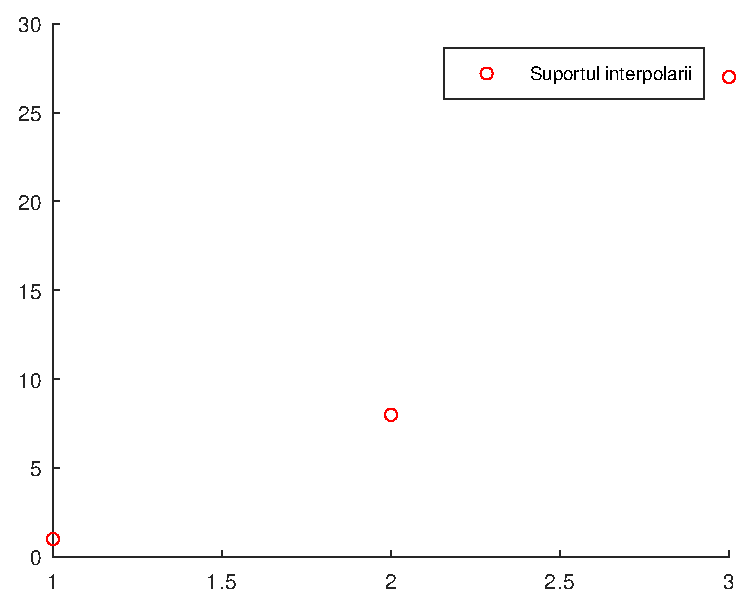
\includegraphics[width=0.85\textwidth]{scatter_ex}
\end{minipage}\hspace{-0.5cm}
{\LARGE$\xrightarrow[Newton]{Interpolare}$}\;\;
\begin{minipage}{0.7\textwidth}
    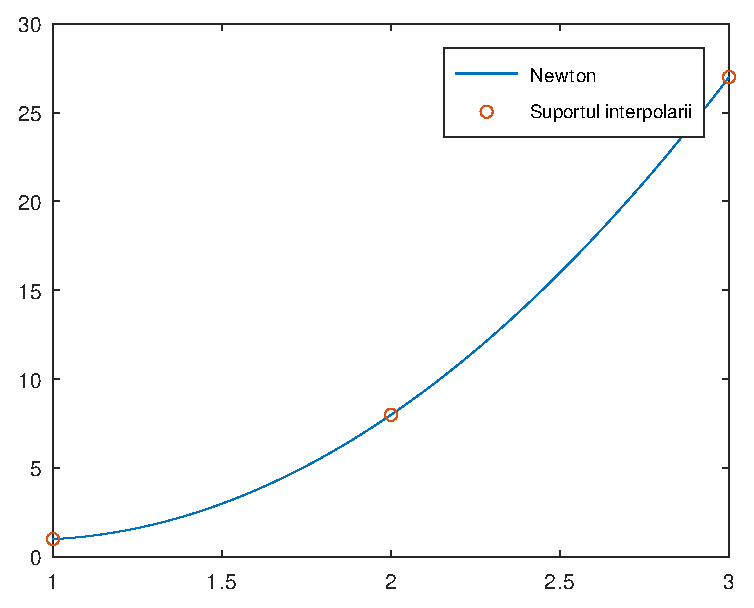
\includegraphics[width=0.5\textwidth]{newton_ex}
\end{minipage}\\


\subsection{Concluzii}
\tab
$\oplus$ Putem adauga incremental puncte noi in suportul interpolarii si avem de calculat doar un coeficient nou $\Rightarrow$ Foarte rapid.\\

$\ominus$ Echivalent cu Lagrange in rest.

\section{Concluzii Interpolarea Polinomiala}
\label{sec:concluzii_polinomiala}

\subsection{Comparatii intre tipurile de interpolare polinomiala}

\begin{center}
    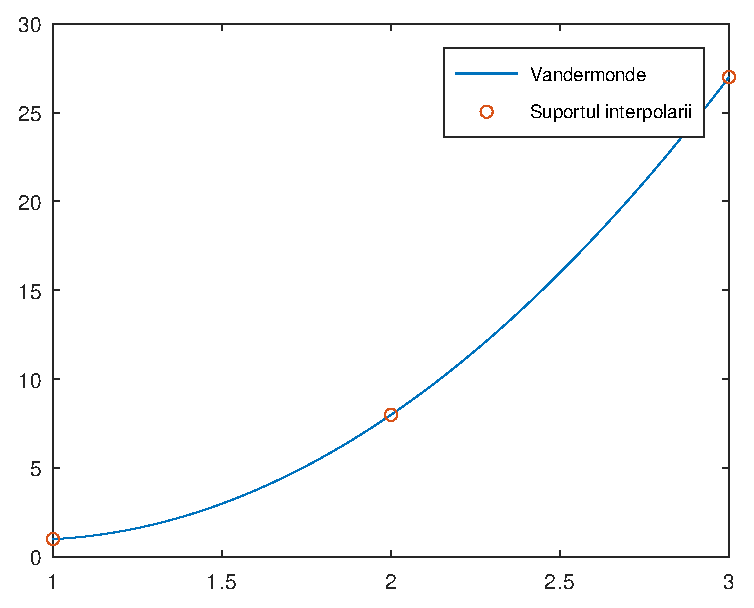
\includegraphics[width=0.25\textwidth]{vandermonde_ex}
    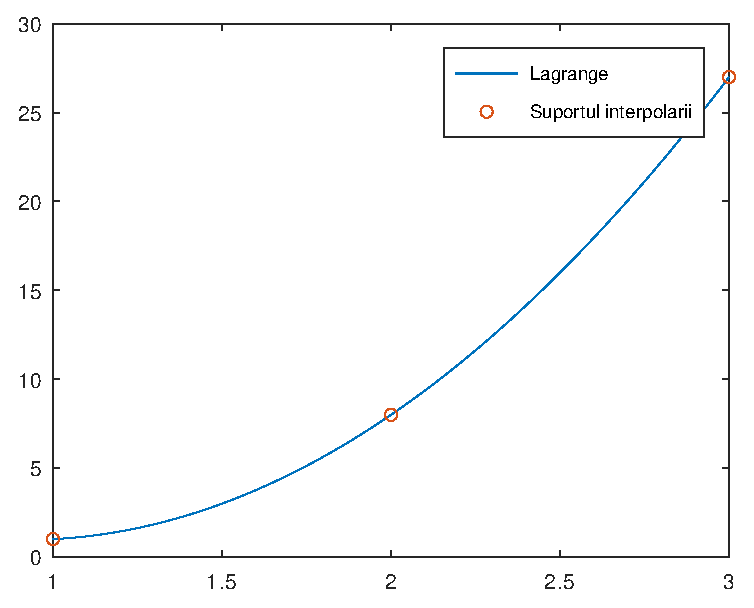
\includegraphics[width=0.25\textwidth]{lagrange_ex}
    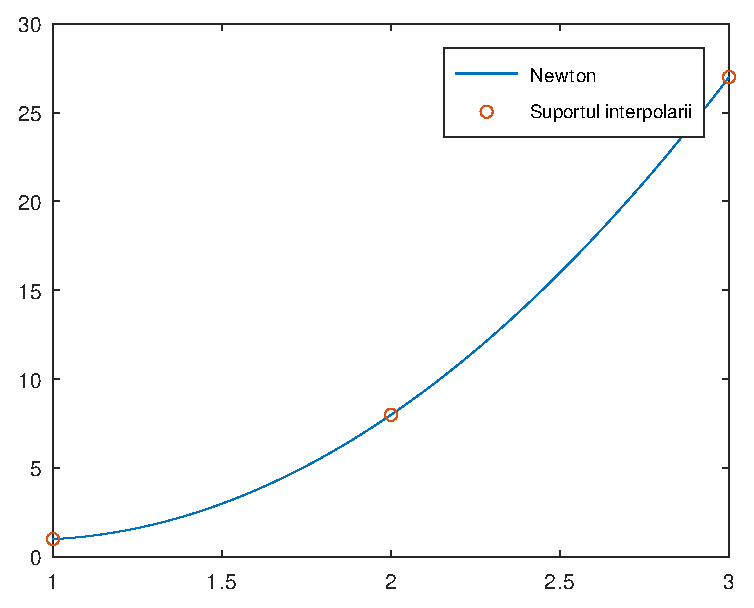
\includegraphics[width=0.25\textwidth]{newton_ex}
\end{center}
\tab Asadar, cele 3 metode de interpolare exemplificate anterior (Vandermonde, Lagrange si Newton) produc acelasi polinom de interpolare, dar prin tehnici diferite.


\subsection{Ce putem imbunatati?}
\begin{itemize}
    \item Asa cum am vazut in exemplele anterioare, gradul polinomului de interpolare creste odata cu cresterea numarului de puncte din suportul interpolarii.
    
    \item Acest lucru conduce la marirea erorii de aproximare si oscilatii ale polinomului de interpolare.
    
    \item Pentru a mentine gradul polinomului de interpolare cat mai mic, introducem in discutie \textit{functiile spline} (functii de grad mic, definite pe subintervale).
\end{itemize}


\section{Introducere Interpolare Cu Functii Spline}
\label{sec:spline}

\subsection{Notiuni generale}
\tab In continuare, consideram o functie $f:[a,b]\rightarrow\mathbb{R}.$
Cunoastem \textbf{valorile functiei} si \textbf{valorile derivatei} intr-un numar redus de puncte $(x_i, f(x_i)), \, i = \overline{0, n}$. Dorim sa interpolam aceste puncte cu o functie spline.\\

\textbf{Functiile spline} sunt functii definite pe subintervale:
$S(x) = \begin{cases}
    S_0(x),\; x \in [x_0, x_1]\\
    S_1(x),\; x \in [x_1, x_2]\\
    \dots\\
    S_i(x),\; x \in [x_i, x_{i+1}]\\
    \dots\\
    S_{n-1}(x),\; x \in [x_{n-1}, x_n]\\
\end{cases}$

\subsection{Motivatie}

\tab Dorim sa eliminam oscilatia polinomului de interpolare, folosind functii de grad mic.

\begin{minipage}{0.65\textwidth}
    Sa consideram ca exemplu functia Heaviside (functia treapta):\\
    Vom interpola pe rand:
    \begin{itemize}
        \item \textit{Polinomial}
        \item Folosind functii \textit{spline liniare}
        \item Folosind functii \textit{spline cubice}
    \end{itemize}
\end{minipage}
\begin{minipage}{0.35\textwidth}
    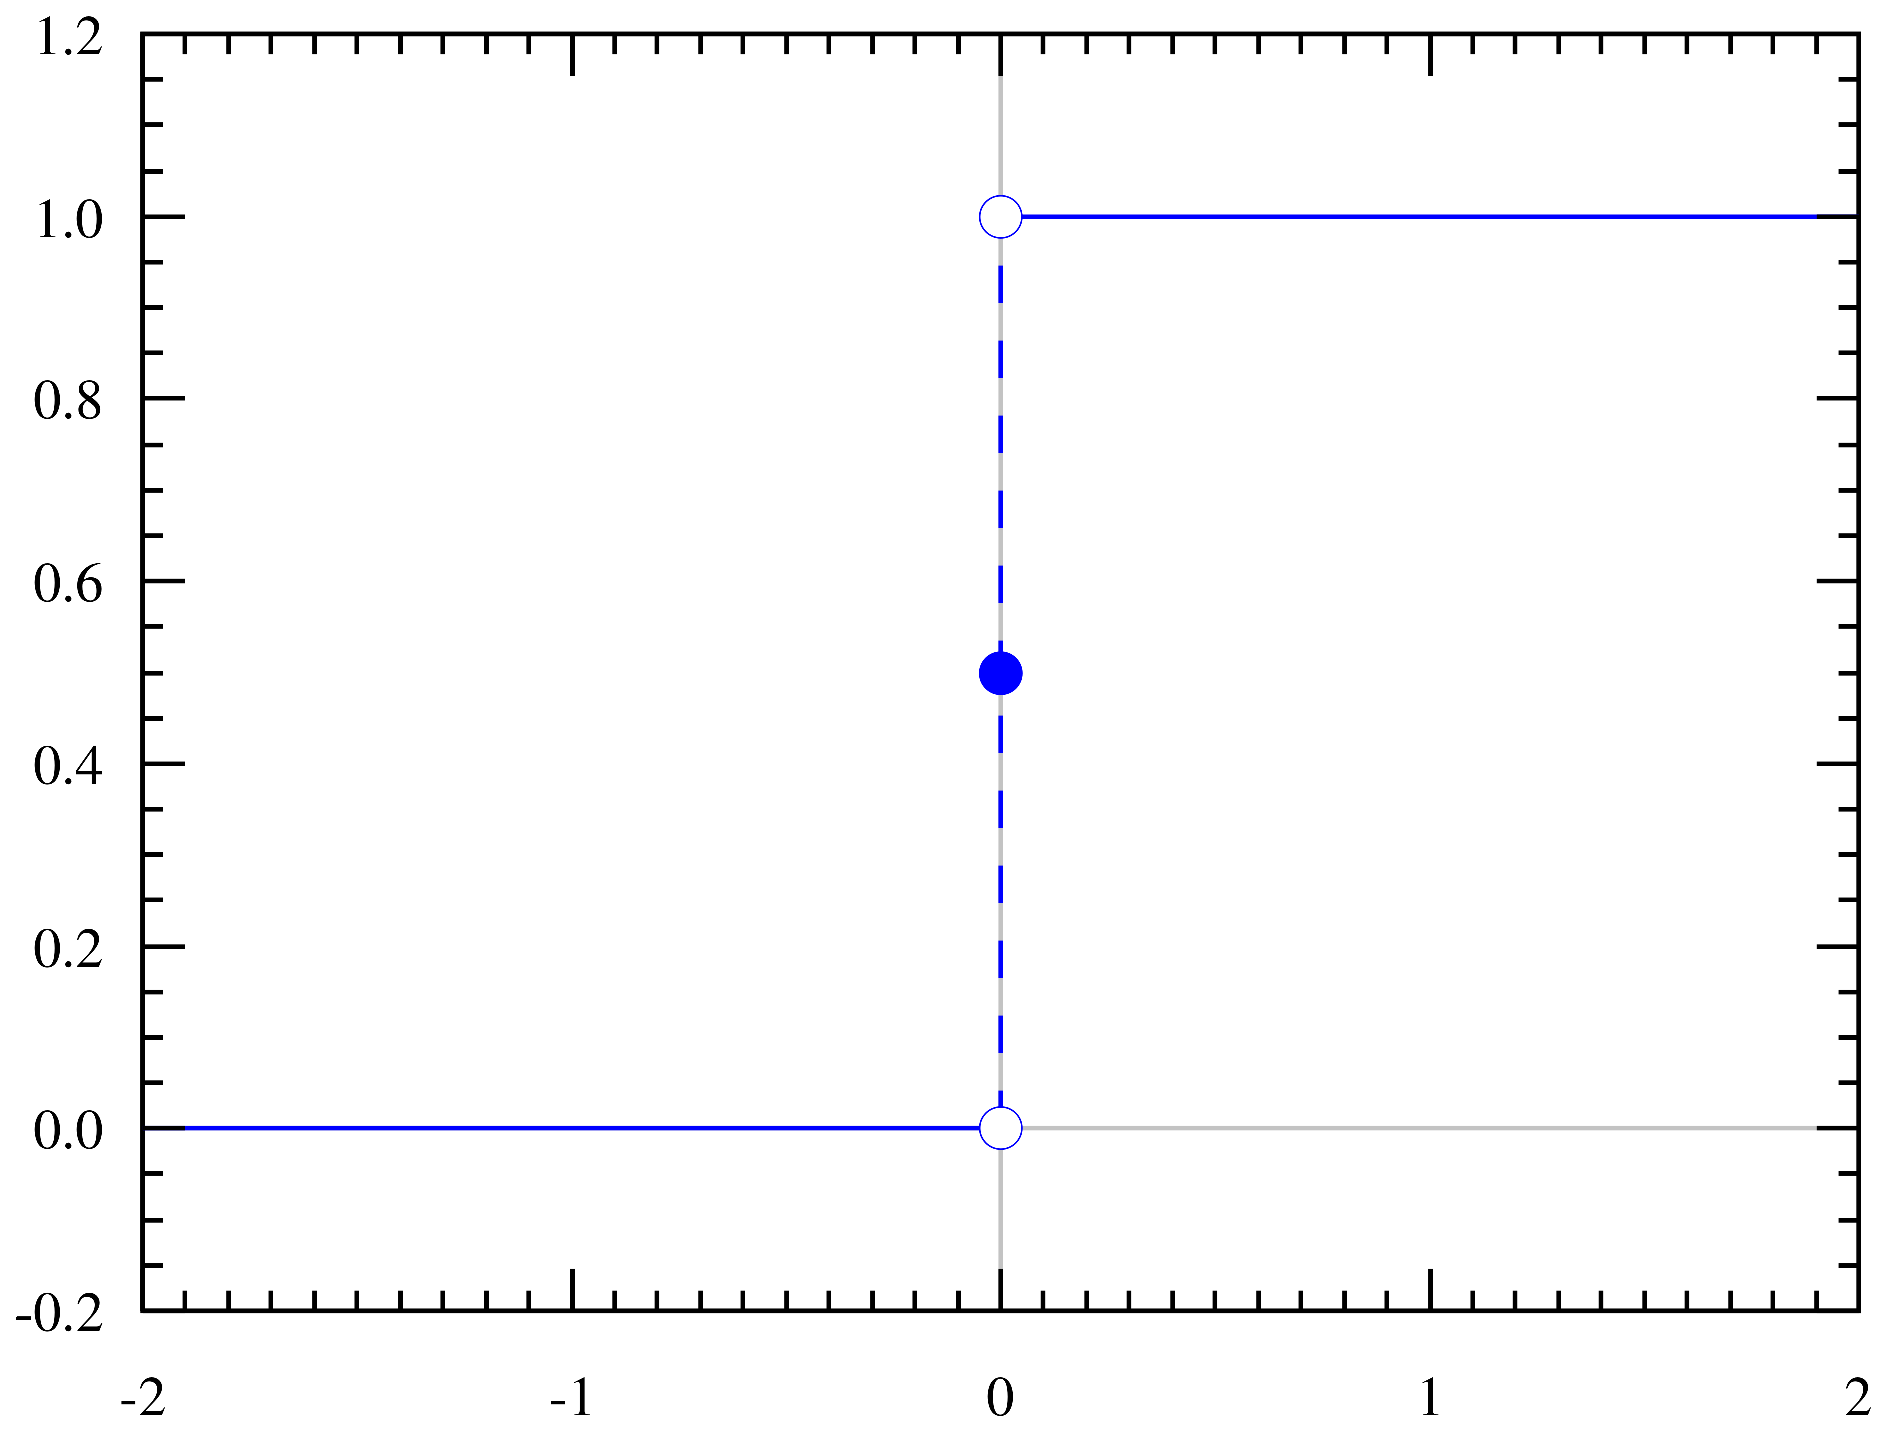
\includegraphics[scale=0.115]{heaviside_fct}
\end{minipage}\\

\begin{center}
    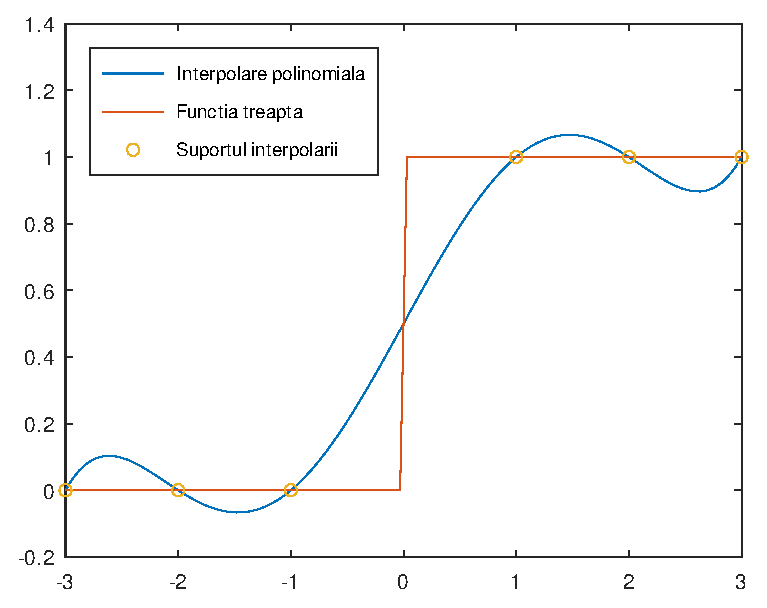
\includegraphics[width=0.275\textwidth]{heaviside_pol}
    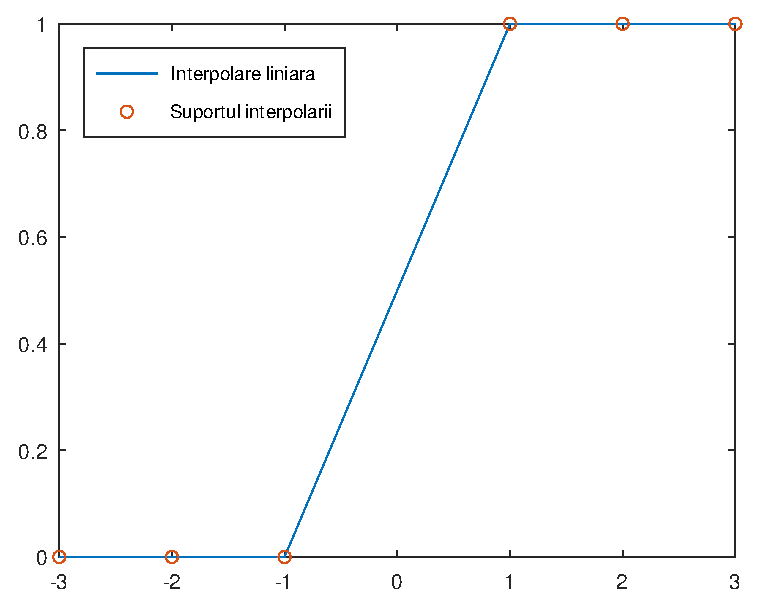
\includegraphics[width=0.275\textwidth]{heaviside_lin}
    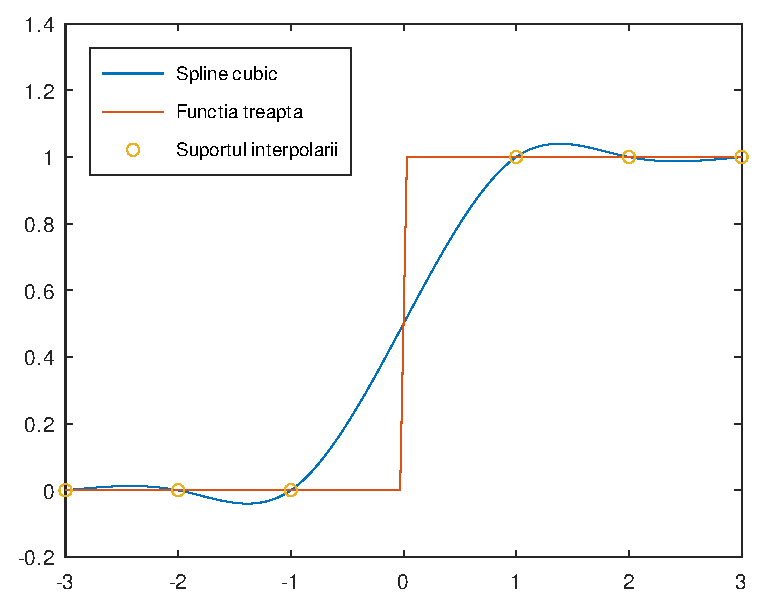
\includegraphics[width=0.275\textwidth]{heaviside_cub}
\end{center}

Daca folosim spline liniar, vom avea $5$ polinoame de gradul I, iar daca folosim spline cubic, vom avea $5$ polinoame de gradul III (cate unul intre fiecare 2 puncte consecutive).

Asadar, putem folosi polinoame de grad I sau III pe subintervale, in loc sa interpolam cu un polinom de grad mare pe tot intervalul. Practic, impartim problema in probleme mai mici.

\section{Interpolare cu functii spline liniare}
\label{sec:liniare}

\subsection{Modul de determinare}
\tab Pornim de la forma generala a functiei spline
$S(x) = \begin{cases}
    S_0(x),\; x \in [x_0, x_1]\\
    \dots\\
    S_i(x),\; x \in [x_i, x_{i+1}]\\
    \dots\\
    S_{n-1}(x),\; x \in [x_{n-1}, x_n]\\
\end{cases}$ \textbf{(**)}\\

Alegem $S_i(x)$ de forma $a_i \cdot x + b_i$, deci o functie liniara.

Asadar, pornim de la forma $S_i(x) = a_i \cdot x + b_i,\; i = 0 : n-1$

Pentru a determina constantele $a_i$ si $b_i$, avem nevoie de $(2 \cdot n)$ ecuatii:

\begin{center}
    \begin{minipage}[t]{0.4\textwidth}
    Conditii de \textbf{interpolare}:\\
        $S_i(x_i) = f(x_i),\; i = 0 : n-1$\\
        $S_{n-1}(x_n) = f(x_n)$
    \end{minipage}
    \begin{minipage}[t]{0.5\textwidth}
        Conditii de \textbf{racordare (de continuitate)}:
        $S_i(x_{i+1}) = S_{i+1}(x_{i+1}),\; i = 0 : n-2$
    \end{minipage}
\end{center}

$\hspace{3cm}\xRightarrow[\text{}]{\text{(\dots)}} \framebox{$\begin{cases}
    a_i = \frac{f(x_{i+1}) - f(x_i)}{x_{i+1} - x_i}\\
    b_i = \frac{x_{i+1} \cdot f(x_i) - x_i \cdot f(x_{i+1})}{x_{i+1} - x_i}
\end{cases},\; i = 0 : n-1$}$

\subsection{Exemplu numeric}
\tab Sa consideram cunoscute urmatoarele puncte din plan: $\{(1,1), (2,2), (3,0), (4,1)\}$:\\

\begin{tabular}{c | c | c | c | c}
    $x$ & 1 & 2 & 3 & 4 \\
    \hline
    $f(x)$ & 1 & 2 & 0 & 1  \\
\end{tabular}
$\Rightarrow$ Avem urmatoarele noduri: $x_0=1;\; x_1=2;\; x_2=3;\; x_3=4$.

Suportul interpolarii este $S=[(1,1), (2,2), (3,0), (4,1)]$.

Particularizand \hyperref[sec:liniare]{\textbf{(**)}}, obtinem spline-ul:
$S(x) = \begin{cases}
  S_0(x),\; x \in [1, 2]\\
  S_1(x),\; x \in [2, 3]\\
  S_2(x),\; x \in [3, 4]\\
\end{cases}$, unde $S_i(x) = a_i \cdot x + b_i$

\begin{minipage}{0.75\textwidth}
    \begin{itemize}
    \item Pentru $i = 0: \begin{cases}
      a_0 = \frac{f(x_1) - f(x_0)}{x_1 - x_0} = \frac{2 - 1}{2 - 1} = 1\\
      b_0 = \frac{x_1 \cdot f(x_0) - x_0 \cdot f(x_1)}{x_1 - x_0} = \frac{2\cdot1 - 1\cdot2}{2 - 1} = 0\\
    \end{cases} \Rightarrow S_0(x) = x$
    \item Pentru $i = 1: \begin{cases}
      a_1 = \frac{f(x_2) - f(x_1)}{x_2 - x_1} = \frac{0 - 2}{3 - 2}  = -2\\
      b_1 = \frac{x_2 \cdot f(x_1) - x_1 \cdot f(x_2)}{x_2 - x_1} = \frac{3\cdot2 - 2\cdot0}{3-2} = 6\\
    \end{cases} \Rightarrow S_1(x) = 6x - 2$
    \item Pentru $i = 2: \begin{cases}
      a_2 = \frac{f(x_3) - f(x_2)}{x_3 - x_2} = \frac{1 - 0}{4 - 3} = 1\\
      b_2 = \frac{x_3 \cdot f(x_2) - x_2 \cdot f(x_3)}{x_3 - x_2} = \frac{4\cdot0 -3\cdot1}{4 - 3} = -3\\
    \end{cases} \Rightarrow S_2(x) = x - 3$
    \end{itemize}
\end{minipage}
\begin{minipage}{0.5\textwidth}
    $\Longrightarrow$ \framebox{$S(x) = \begin{cases}
      x,\; x \in [1, 2]\\
      6 \cdot x - 2,\; x \in [2, 3]\\
      x - 3,\; x \in [3, 4]
    \end{cases}$\\
    }
\end{minipage}

\begin{center}
    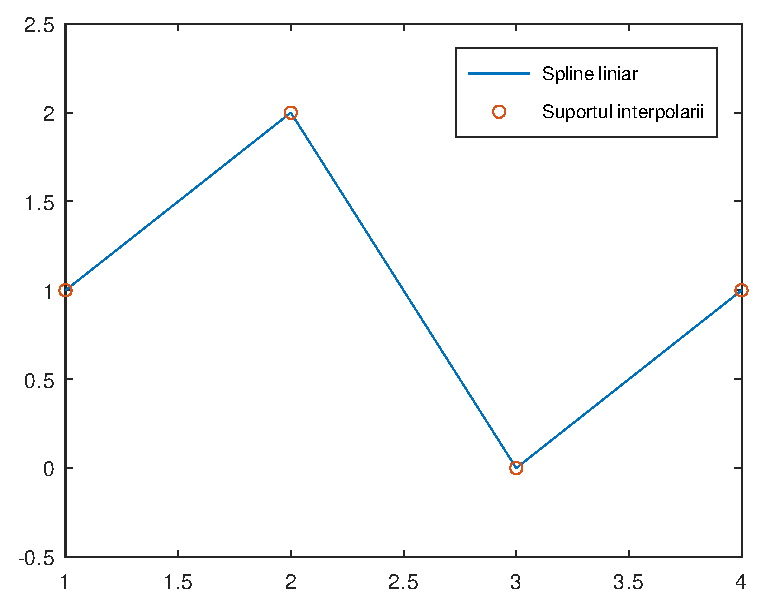
\includegraphics[scale=0.5]{liniara_ex}
\end{center}

\subsection{Concluzii}
\tab
$\oplus$ Dispare fenomenul de oscilatie prin mentinerea gradului polinomului de interpolare mic.\\

$\ominus$ Derivata de ordin I nu este o functie continua $\iff$ Nu se face o trecere neteda in capetele subintervalelor.\\


\section{Interpolare cu functii spline cubice C1}
\label{sec:spline_c1}

\subsection{De ce spline-uri cubice?}

\begin{minipage}{0.75\textwidth}
    \tabto{0.5cm} Tinand cont ca am discutat despre spline-uri \textit{liniare} si acum discutia se indreapta catre spline-uri \textit{cubice}, intrebarea fireasca este \textit{"De ce cubice si nu patratice?"}. La nivel simplist, raspunsul este simplu: Folosim spline-uri cubice in locul celor patratice, deoarce:
    \begin{itemize}
        \item $3$ este cel mai mic grad al unui polinom care permite o \textit{inflexiune}.
        \item $3$ nu este un grad foarte mare $\Rightarrow$ Polinomul de interpolare \textit{nu oscileaza} in capete.
    \end{itemize}
\end{minipage}
\hspace{0.75cm}\begin{minipage}{0.25\textwidth}
    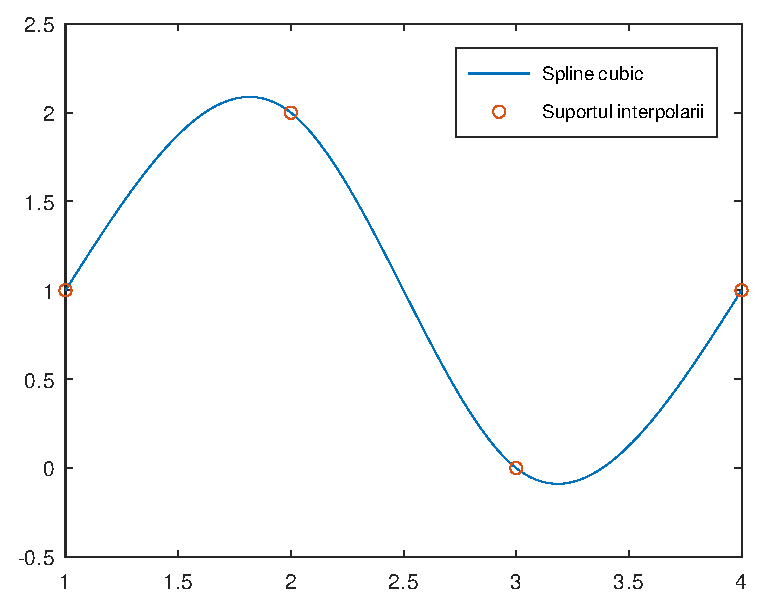
\includegraphics[width=1.25\textwidth]{cubic_ex}
\end{minipage}


\subsection{Modul de determinare}
\label{sec:determinare_c1}

\tab La modul general, o functie spline cubica scrisa in functie de $x-x_i$, arata astfel:

\framebox{$S_i(x) = a_i + b_i \cdot (x-x_i) + c_i \cdot (x-x_i)^2 + d_i \cdot (x-x_i)^3,\; i = 0 : n-1$}\\

Se pune problema determinarii coeficientilor $a_i, b_i, c_i, d_i$. Spline-urile de clasa $C^1$ necesita cunoasterea derivatei in suportul interpolarii. Asadar, pentru a determina coeficientii, punem conditii de \textit{interpolare} (de tip Hermite) si conditii de \textit{racordare}:\\\\

\begin{itemize}
    \item Conditii de \textit{interpolare} de tip Hermite:
    \begin{itemize}
        \item Fiecare spline trece prin punctul sau de interpolare:
        \framebox{$\begin{cases}
            S_i(x) = f(x_i),\; i = 0 : n-1\\
            S_{n-1}(x_n) = f(x_n)
        \end{cases}$}
        \\$\Rightarrow (n+1)$ ecuatii
        
        \item Fiecare spline are aceeasi panta cu functia pe care o aproximeaza:
        \framebox{$\begin{cases}
            S_i'(x) = f'(x_i),\; i = 0 : n-1\\
            S_{n-1}'(x_n) = f'(x_n)
        \end{cases}$}
        \\$\Rightarrow (n+1)$ ecuatii
    \end{itemize}
    
    \item Conditii de \textit{racordare}:
    \begin{itemize}
        \item Racordam functiile (Unde se termina $S_i$, incepe $S_{i+1}$): \framebox{$S_i(x_{i+1}) = S_{i+1}(x_{i+1}),\; i = 0 : n-2$}\\
        \\$\Rightarrow (n-1)$ ecuatii
        
        \item Spline-urile au aceeasi panta in punctele de contact: \framebox{$S_i'(x_{i+1}) = S_{i+1}'(x_{i+1}),\; i = 0 : n-2$}\\
        \\$\Rightarrow (n-1)$ ecuatii
    \end{itemize}

\end{itemize}

Din conditiile de mai sus, obtinem $(4 \cdot n)$ ecuatii.

Astfel, putem sa determinam cele $(4 \cdot n)$ necunoscute ($a_i, b_i, c_i, d_i,\; i = 0 : n-1$).

\subsection{Forma parametrica}
\tab Pentru a ne apropia de o rezolvare \textit{computationala}, introducem forma parametrica a functiei spline cubice.

Pornim de la forma generala a spline-ului cubic: $S_i(x) = a_i + b_i \cdot (x-x_i) + c_i \cdot (x-x_i)^2 + d_i \cdot (x-x_i)^3$ si notam $x-x_i = h_i \cdot t \iff t = \frac{x-x_i}{h_i} \;$, unde  $h_i = x_{i+1} - x_i\;$ (lungimea intervalului\;$[x_i, x_{i+1}]$) si $t \in [0, 1]$.

$\Rightarrow S_i(t) = a_i + b_i \cdot h_i \cdot t + c_i \cdot h_i^2 \cdot t^2 + d_i \cdot h_i^3 \cdot t^3$.\\

Asadar, la modul general, forma parametrica a unei functii spline cubice, arata astfel:

\framebox{$S_i(t) = a_i + b_i \cdot h_i \cdot t + c_i \cdot h_i^2 \cdot t^2 + d_i \cdot h_i^3 \cdot t^3$}, unde:
$\begin{cases}
  t \in [0, 1]\\
  i = 0 : n-1\\
  h_i = x_{i+1} - x_i\; $(lungimea intervalului\;$[x_i, x_{i+1}]$)$\\
\end{cases}$

\subsection{Polinoamele Bernstein}

\tab Introducem in cadrul discutiei \textbf{polinoamele Bernstein}\framebox[0.3cm][r]{\footnotemark} de grad $n$, deoarece sunt utilizate pentru a eficientiza procesul de calculare al coeficientilor functiilor spline cubice in forma parametrica.

\footnotetext{\framebox[8.25cm]{\url{https://mathworld.wolfram.com/BernsteinPolynomial.html}}}

\framebox{$B_{i,n}(t) \; \eqdef \; C_n^i \cdot (1-t)^{n-i} \cdot t^i$},$\; t \in [0, 1],\; i = \overline{0, n}$.\\

Pentru a intelege mai bine, exemplificam primele polinoame:\\

\begin{minipage}[b]{0.5\textwidth}
    Grad $0$: $B_{0,0}(t) = C_0^0 \cdot (1-t)^{0-0} \cdot t^0 = 1$\\\\
    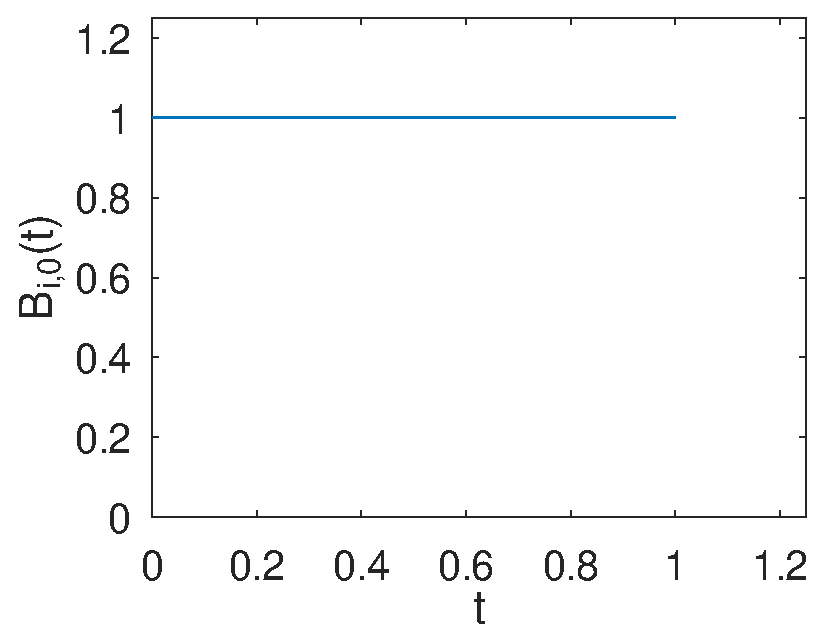
\includegraphics[scale=0.5]{bernstein_0}
\end{minipage}
\hspace{0.75cm}\begin{minipage}[b]{0.5\textwidth}
    Grad $1$:
    $\begin{cases}
      B_{0,1}(t) = C_1^0 \cdot (1-t)^{1-0} \cdot t^0 = 1-t\\
      B_{1,1}(t) = C_1^1 \cdot (1-t)^{1-1} \cdot t^1 = t\\
    \end{cases}$
    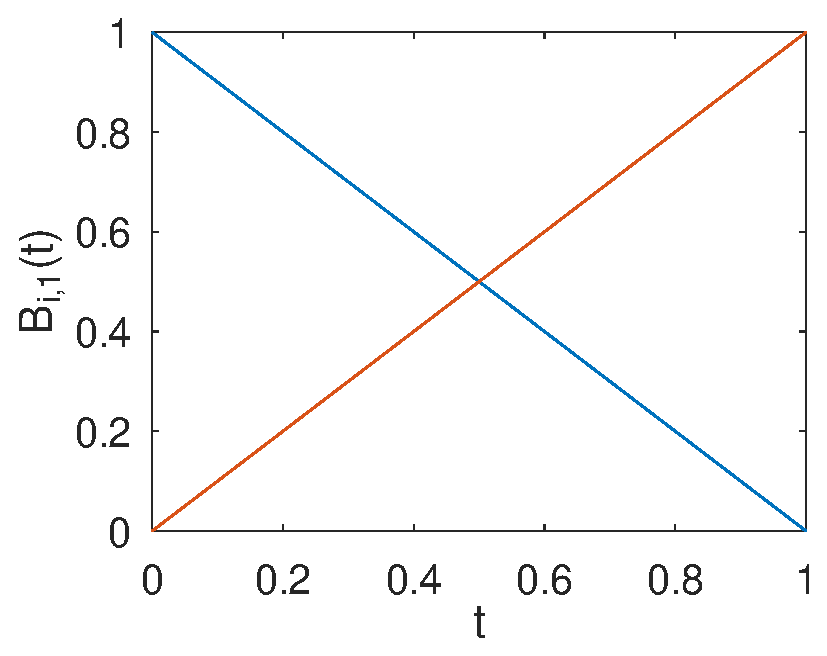
\includegraphics[scale=0.5]{bernstein_1}
\end{minipage}\\
\begin{minipage}[b]{0.5\textwidth}
    Grad $2$:
    $\begin{cases}
      B_{0,2}(t) = C_2^0 \cdot (1-t)^{2-0} \cdot t^0 = (1-t)^2\\
      B_{1,2}(t) = C_2^1 \cdot (1-t)^{2-1} \cdot t^1 = 2 \cdot (1-t) \cdot t\\
      B_{2,2}(t) = C_2^2 \cdot (1-t)^{2-2} \cdot t^2 = t^2\\
    \end{cases}$
    \begin{center}
        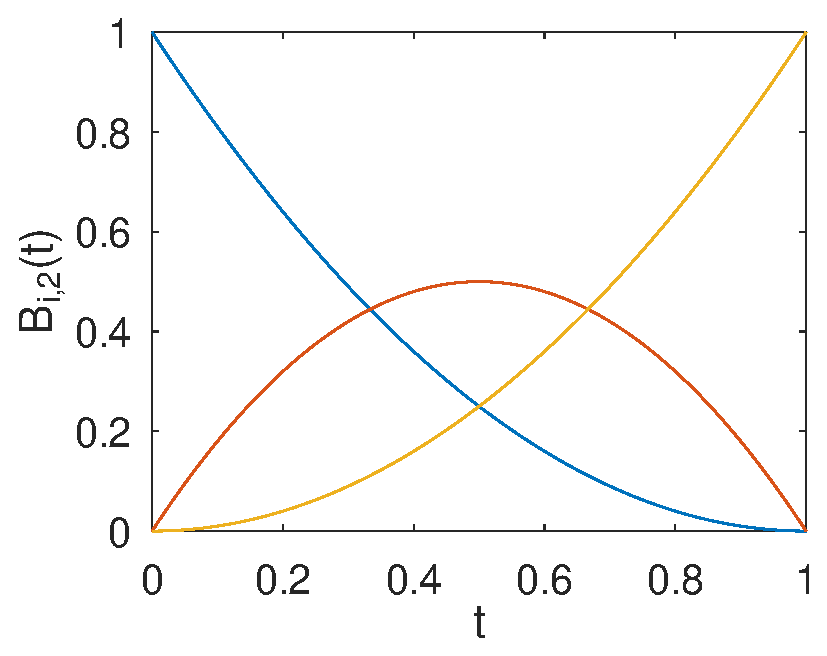
\includegraphics[scale=0.5]{bernstein_2}
    \end{center}
\end{minipage}
\hspace{0.75cm}\begin{minipage}[b]{0.5\textwidth}
    Grad $3$:
    $\begin{cases}
      B_{0,3}(t) = C_3^0 \cdot (1-t)^{3-0} \cdot t^0 = (1-t)^3\\
      B_{1,3}(t) = C_3^1 \cdot (1-t)^{3-1} \cdot t^1 = 3 \cdot (1-t)^2 \cdot t\\
      B_{2,3}(t) = C_3^2 \cdot (1-t)^{3-2} \cdot t^2 = 3 \cdot (1-t) \cdot t^2\\
      B_{3,3}(t) = C_3^3 \cdot (1-t)^{3-3} \cdot t^3 = t^3\\
    \end{cases}$
    \begin{center}
        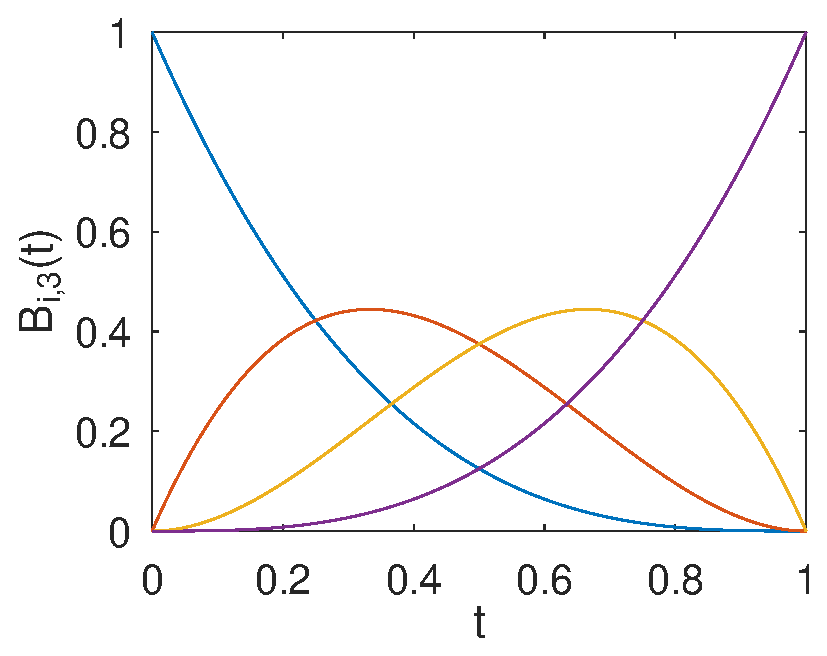
\includegraphics[scale=0.5]{bernstein_3}
    \end{center}
\end{minipage}

Folosind polinoamele Bernstein de grad $n = 3$, obtinem forma parametrica a spline-ului cu care vom lucra de acum inainte:\\

\framebox{$S_i(t) = a_i' \cdot (1-t)^3 + b_i' \cdot 3 \cdot t \cdot (1-t)^2 + c_i' \cdot 3 \cdot t^2 \cdot (1-t) + d_i' \cdot t^3,\; i = 0 : n-1,\; t \in [0, 1]$}\\

$\xRightarrow[\text{prezentate anterior}]{\text{Se impun conditiile }}\;$
\framebox{$\begin{cases}
  a_i' = f(x_i),\; i = 0 : n-1\\
  d_i' = f(x_{i+1}),\; i = 0 : n-1\\
  c_i' = f(x_{i+1}) - \frac{h_i}{3} \cdot f'(x_{i+1}),\; i = 0 : n-1\\
  b_i' = f(x_i) + \frac{h_i}{3} \cdot f'(x_i),\; i = 0 : n-1
\end{cases}$}

In cele din urma, forma in variabila $x$ pentru fiecare functie spline cubica de clasa $C^1$ se obtine prin \textit{schimbarea de variabila} \framebox{$t = \frac{x-x_i}{h_i}$}

\subsection{Exemplu numeric}
\tab Sa consideram cunoscute urmatoarele puncte din plan:
\begin{tabular}{c | c | c | c}
    $x$ & 1 & 2 & 4 \\
    \hline
    $f(x)$ & 3 & 4 & 6 \\
    \hline
    $f'(x)$ & 0 & 2 & 5 \\
\end{tabular}\\

$\Rightarrow$ Avem urmatoarele noduri: $x_0=1;\; x_1=2;\; x_2=4$.

Tinand cont de forma unei functii spline, putem particulariza pe exemplul nostru: $S(x) = $
$\begin{cases}
  S_0(x),\; x \in [1, 2] \\
  S_1(x),\; x \in [2, 4]
\end{cases}$

\subsubsection{Metoda 1 - Utilizand forma generala}
\tab Avem $n = 3$ puncte in suportul interpolarii, deci vom avea $2$ subintervale.

Pornim de la forma generala a functiei spline si derivam expresia:\\

\framebox{$S_i(x) = a_i + b_i \cdot (x-x_i) + c_i \cdot (x-x_i)^2 + d_i \cdot (x-x_i)^3,\; i = 0 : 1$} $|()'$ \vspace{0.1cm}
\tabto{0.5cm} $S'_i(x) = b_i + 2 \cdot c_i \cdot (x-x_i) + 3 \cdot d_i \cdot (x-x_i)^2,\; i = 0 : 1$\\

\begin{itemize}
    \item Punem conditiile de \textit{interpolare} de tip Hermite:
    \begin{itemize}
        \item Fiecare spline trece prin punctul sau de interpolare:
        $\begin{cases}
            S_0(x_0) = f(x_0) \iff S_0(1) = f(1) = 3 \\
            S_1(x_1) = f(x_1) \iff S_1(2) = f(2) = 4 \\
            S_1(x_2) = f(x_2) \iff S_1(4) = f(4) = 6 \\
        \end{cases}$
        
        \item Fiecare spline are aceeasi panta cu functia pe care o aproximeaza:
        $\begin{cases}
            S_0'(x_0) = f'(x_0) \iff S_0'(1) = f'(1) = 0 \\
            S_1'(x_1) = f'(x_1) \iff S_1'(2) = f'(2) = 2 \\
            S_1'(x_2) = f'(x_2) \iff S_1'(4) = f'(4) = 5 \\
        \end{cases}$
    \end{itemize}
    
    \item Punem conditiile de \textit{racordare}:
    \begin{itemize}
        \item Racordam functiile (Unde se termina $S_0$, incepe $S_1$):
        $S_0(x_1) = S_1(x_1) \iff S_0(2) = S_1(2) = 4$
        
        \item Spline-urile au aceeasi panta in punctele de contact: $S_0'(x_1) = S_1'(x_1) \iff S_0'(2) = S_1'(2) = 2$
    \end{itemize}
\end{itemize}


Se rezolva sistemul de $8$ ecuatii cu $8$ necunoscute $\Longrightarrow$ Coeficientii:
$\begin{cases}
  a_0 = 3 \\
  b_0 = 0 \\
  c_0 = 1 \\
  d_0 = 0 \\
\end{cases}$;\;
$\begin{cases}
  a_1 = 4 \\
  b_1 = 2 \\
  c_1 = -3 \\
  d_1 = \frac{5}{4} \\
\end{cases}$\vspace{0.3cm}

$\Longrightarrow$
\begin{minipage}{0.65\textwidth}
    \framebox{$S(x) = \begin{cases}
        3 + 0 \cdot (x-1) + 1 \cdot (x-1)^2 + 0 \cdot (x-1)^3,\; x \in [1, 2] \\
        4 + 2 \cdot (x-2) -3 \cdot (x-2)^2 + \frac{5}{4} \cdot (x-2)^3,\; x \in [2, 4] \\
    \end{cases}$}
\end{minipage}
\begin{minipage}{0.35\textwidth}
    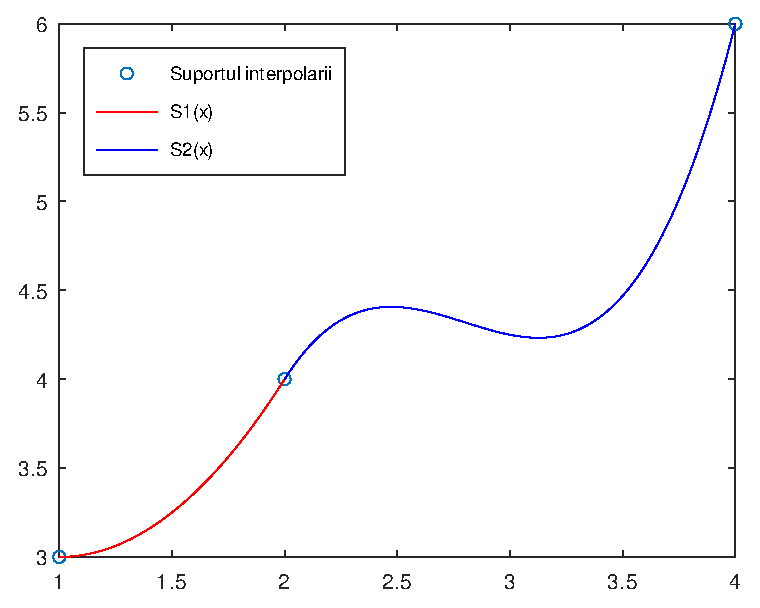
\includegraphics[scale=0.35]{spline_c1_ex}
\end{minipage}\\


\subsubsection{Metoda 2 - Utilizand forma parametrica}

\tab Pornim de la forma parametrica dedusa cu ajutorul polinoamelor Bernstein de grad $3$:\\

$S_i(t) = a_i' \cdot (1-t)^3 + b_i' \cdot 3 \cdot t \cdot (1-t)^2 + c_i' \cdot 3 \cdot t^2 \cdot (1-t) + d_i' \cdot t^3,\; i = 0 : n-1,\; t \in [0, 1]$\\

De data aceasta, pentru determinarea coeficientilor, folosim formulele:\;
$\begin{cases}
  a_i' = f(x_i),\; i = 0 : n-1\\
  d_i' = f(x_{i+1}),\; i = 0 : n-1\\
  c_i' = f(x_{i+1}) - \frac{h_i}{3} \cdot f'(x_{i+1}),\; i = 0 : n-1\\
  b_i' = f(x_i) + \frac{h_i}{3} \cdot f'(x_i),\; i = 0 : n-1
\end{cases}$\\

Tinem cont de faptul ca
$\begin{cases}
  h_0 = x_1 - x_0 = 2 - 1 = 1 \\
  h_1 = x_2 - x_1 = 4 - 2 = 2 \\
\end{cases}$\\

Aplicam formulele mentionate anterior si obtinem coeficientii:\\

$\begin{cases}
  a_0' = f(x_0) = f(1) = 3 \\
  a_1' = f(x_1) = f(2) = 4 \\
\end{cases}$
\hspace{2.575cm}$\begin{cases}
  d_0' = f(x_1) = f(2) = 4 \\
  d_1' = f(x_2) = f(4) = 6 \\
\end{cases}$\\


$\begin{cases}
  c_0' = f(x_1) - \frac{h_0}{3} \cdot f'(x_1) = 4 - \frac{1}{3} \cdot 2 = \frac{10}{3} \\
  c_1' = f(x_2) - \frac{h_1}{3} \cdot f'(x_2) = 6 - \frac{2}{3} \cdot 5 = \frac{8}{3} \\
\end{cases}$
$\begin{cases}
  b_0' = f(x_0) + \frac{h_0}{3} \cdot f'(x_0) = 3 + \frac{1}{3} \cdot 0 = 3 \\
  b_1' = f(x_1) + \frac{h_1}{3} \cdot f'(x_1) = 4 + \frac{2}{3} \cdot 2 = \frac{16}{3} \\
\end{cases}$\\


\tabto{0.5cm} Deci, pentru primul spline: $S_0(t)$, avem coeficientii: $a'_0 = 3,\; b'_0 = 3,\; c'_0 = \frac{10}{3},\; d'_0 = 4$.

Facand schimbarea de variabila: $t = \frac{x-x_0}{h_0} \iff t = \frac{x-1}{1} \iff$ \framebox{$t = x - 1$}


$\Longrightarrow$ \framebox{$S_0(x) = 3 \cdot (2-x)^3 + 9 \cdot (x-1) \cdot (2-x)^2 + 10 \cdot (x-1)^2 \cdot (2-x) + 4 \cdot (x-1)^3,\; x \in [1, 2]$}\\


Procedand in mod analog, obtinem:

$\Longrightarrow$ \framebox{$S_1(x) = 4 \cdot (\frac{4-x}{3})^3 + 16 \cdot (\frac{x-2}{2}) \cdot (\frac{4-x}{2})^2 + 8 \cdot (\frac{x-1}{2})^2 \cdot (\frac{4-x}{2}) + 6 \cdot (\frac{x-2}{2})^3,\; x \in [2, 4]$}\\


In forma finala, functia spline cubica de clasa $C^1$ care interpoleaza cele 3 puncte din exemplul nostru, arata astfel:\\

\framebox{$S(x) = $
$\begin{cases}
    S_0(x) = 3 \cdot (2-x)^3 + 9 \cdot (x-1) \cdot (2-x)^2 + 10 \cdot (x-1)^2 \cdot (2-x) + 4 \cdot (x-1)^3,\; x \in [1, 2]\\
    
    S_1(x) = 4 \cdot (\frac{4-x}{3})^3 + 16 \cdot (\frac{x-2}{2}) \cdot (\frac{4-x}{2})^2 + 8 \cdot (\frac{x-1}{2})^2 \cdot (\frac{4-x}{2}) + 6 \cdot (\frac{x-2}{2})^3,\; x \in [2, 4]
\end{cases}$}\\

Asa cum ne-am fi asteptat, in mod evident, cele 2 metode converg la aceeasi functie spline cubica, diferenta fiind facuta de modul in care se ajunge la rezultat.

\subsection{Concluzii}

\tab
$\oplus$ Dispare fenomenul de oscilatie prin mentinerea gradului polinomului de interpolare mic.\\

$\oplus$ De data aceasta, in capetele intervalelor se face o trecere neteda, deoarce se impun niste conditii de racordare mai puternice.\\

$\ominus$ Este necesar sa se cunoasca valorile derivatei I in punctele din suportul interpolarii. \\

\section{Interpolare cu functii spline cubice C2}
\label{sec:spline_c2}

\subsection{Modul de determinare}
\tab Pornim de la forma generala: \framebox{$S_i(x) = a_i + b_i \cdot (x-x_i) + c_i \cdot (x-x_i)^2 + d_i \cdot (x-x_i)^3,\; i = 0 : n-1$}\\

Comparativ cu cele de clasa $C^1$, functiile spline de clasa $C^2$ au proprietatea ca sunt derivabile de $2$ ori si au derivatele continue.

Vom deduce in cele ce urmeaza conditiile care trebuie puse pentru a determina coeficientii $a_i, b_i, c_i, d_i$:


\begin{itemize}
    \item Conditii de \textit{interpolare} de tip Lagrange:
    \begin{itemize}
        \item Fiecare spline trece prin punctul sau de interpolare:
        \framebox{$\begin{cases}
            S_i(x_i) = f(x_i), i = 0 : n-1 \\
            S_{n-1}(x_n) = f(x_n)
        \end{cases}$}
        \\$\Rightarrow (n+1)$ ecuatii
    \end{itemize}
    
    \item Conditii de \textit{racordare}:
    \begin{itemize}
        \item Racordam functiile (Asiguram continuitatea $C^0$):
        \framebox{$S_i(x_{i+1}) = S_{i+1}(x_{i+1}), i = 0 : n-2$}
        \\$\Rightarrow (n-1)$ ecuatii
        
        \item Functiile au aceeasi \textit{panta} in punctele de contact (Asiguram $C^1$):
        \framebox{$S'_i(x_{i+1}) = S'_{i+1}(x_{i+1}), i = 0 : n-2$}
        \\$\Rightarrow (n-1)$ ecuatii
        
        \item Functiile au aceeasi \textit{convexitate} in punctele de contact (Asiguram $C^2$):
        \framebox{$S''_i(x_{i+1}) = S''_{i+1}(x_{i+1}), i = 0 : n-2$}
        \\$\Rightarrow (n-1)$ ecuatii
    \end{itemize}
    
    \item Pana acum avem $(n+1) + 3 \cdot (n-1) = 4n - 2$ ecuatii, pentru $4n$ necunoscute. Pentru ultimele 2 ecuatii, putem pune urmatoarele conditii in \textit{capete}, in functie de tipul de spline ales:
    
    \begin{minipage}{0.5\textwidth}
        \begin{itemize}
            \item Spline \textbf{natural}:
            \framebox{$\begin{cases}
                S''_0(x_0) = 0 \\
                S''_{n-1}(x_n) = 0 \\
            \end{cases}$}
        
            \item Spline \textbf{tensionat}:
            \framebox{$\begin{cases}
                S'_0(x_0) = f'(x_0) \\
                S'_{n-1}(x_n) = f'(x_n) \\
            \end{cases}$}
        \end{itemize}
    \end{minipage}
    \begin{minipage}{0.6\textwidth}
        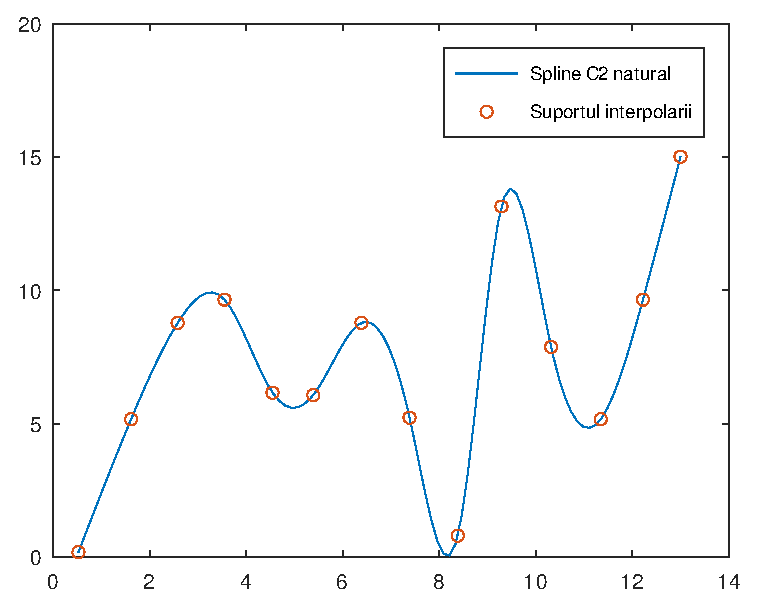
\includegraphics[width=0.6\textwidth]{spline_c2_nat}
    \end{minipage}

\end{itemize}

Astfel, am cumulat $(4n-2) + 2 = 4n$ ecuatii pentru $4n$ necunoscute.

Observatie: Spline-ul \textit{tensionat} ofera o aproximare mai buna, insa necesita cunoasterea derivatei I in capetele suportului de interpolare.\\

Din punct de vedere al automatizarii, conditiile care trebuie puse nu sunt de folos. Astfel, prelucrand ecuatiile obtinute prin punerea conditiilor, obtinem urmatoarele relatii:

Coeficientii functiilor spline cubice de clasa $C^2$ sunt dati de relatiile:

\framebox{$a_i = f(x_i),\; i = 0:n$} \\

\framebox{$d_i = \frac{c_{i+1} - c_i}{3 \cdot h_i},\; i = 0 : n-1$} \\

\framebox{$b_i = \frac{a_{i+1} - a_i}{h_i} - \frac{h_i}{3} \cdot (2 \cdot c_i + c_{i+1}),\; i = 0 : n-1$}\\

Coeficientii \framebox{$c_i,\; i = 0 : n-1$} se obtin prin rezolvarea unui sistem \textit{tridiagonal} de forma:\\

\begin{itemize}
    \item Pentru spline $\mathbf{C^2}$ \textbf{natural}:
\end{itemize}
\hspace{-2cm}$\begin{bmatrix}
    \mathbf{1} & \mathbf{0} & 0 & \dots & \dots & 0 \\\\
    \mathbf{h_0} & \mathbf{2(h_0+h_1)} & \mathbf{h1} & \dots  & \dots & \vdots \\\\
    0 & \mathbf{h_1} & \mathbf{2(h_1+h_2)} & \mathbf{h_2} & \dots & 0 \\
     & \dots & \dots & \dots & \dots & \dots \\
    \vdots & \dots & \dots & \mathbf{h_{n-2}} & \mathbf{2(h_{n-2}+h_{n-1})} & \mathbf{h_{n-1}} \\\\
    0 & \dots & \dots & 0 & \mathbf{0} & \mathbf{1} \\
\end{bmatrix}$
$\cdot$
$\begin{bmatrix}
    0 \\
    \frac{3}{h_1}(a_2-a_1) - \frac{3}{h_0}(a_1-a_0) \\
    \vdots \\
    \frac{3}{h_{n-1}}(a_n-a_{n-1}) - \frac{3}{h_{n-2}}(a_{n-1}-a_{n-2}) \\
    0 \\
\end{bmatrix}$
$=$
$\begin{bmatrix}
    c_0 \\
    c_1 \\
    \vdots \\
    c_n \\
\end{bmatrix}$\\

\begin{itemize}
    \item Pentru spline $\mathbf{C^2}$ \textbf{tensionat}:
\end{itemize}
\hspace{-2.35cm}$\begin{bmatrix}
    \mathbf{2h_0} & \mathbf{h_0} & 0 & \dots & \dots & 0 \\\\
    \mathbf{h_0} & \mathbf{2(h_0+h_1)} & \mathbf{h1} & \dots  & \dots & \vdots \\\\
    0 & \mathbf{h_1} & \mathbf{2(h_1+h_2)} & \mathbf{h_2} & \dots & 0 \\
     & \dots & \dots & \dots & \dots & \dots \\
    \vdots & \dots & \dots & \mathbf{h_{n-2}} & \mathbf{2(h_{n-2}+h_{n-1})} & \mathbf{h_{n-1}} \\\\
    0 & \dots & \dots & 0 & \mathbf{h_{n-1}} & \mathbf{2h_{n-1}} \\
\end{bmatrix}$
$\cdot$
$\begin{bmatrix}
    \frac{3}{h_0}(a_1-a_0) - 3f'(a) \\
    \frac{3}{h_1}(a_2-a_1) - \frac{3}{h_0}(a_1-a_0) \\
    \vdots \\
    \frac{3}{h_{n-1}}(a_n-a_{n-1}) - \frac{3}{h_{n-2}}(a_{n-1}-a_{n-2}) \\
    3f'(b) - \frac{3}{h_{n-1}}(a_n-a_{n-1})
\end{bmatrix}$
$=$
$\begin{bmatrix}
    c_0 \\
    c_1 \\
    \vdots \\
    c_n \\
\end{bmatrix}$\\\\

\noindent Observatie: Functia spline $S_n$ a fost introdusa pentru a ajuta la calcuarea functiilor spline $S_i,\; i = 0 : n-1$.


\subsection{Exemplu numeric}
\tab Sa consideram cunoscute urmatoarele puncte din plan:
\begin{tabular}{c | c | c | c | c}
    $x$ & -1 & 0 & 1 & 2 \\
    \hline
    $f(x)$ & -2 & -1 & 2 & 4 \\
    \hline
    $f'(x)$ & 3 & & & 2 \\
\end{tabular}\\

$\Rightarrow$ Avem urmatoarele noduri: $x_0=-1;\; x_1=0;\; x_2=1;\; x_3=2$.

Tinand cont de forma unei functii spline, putem particulariza pe exemplul nostru: $S(x) = $
$\begin{cases}
  S_0(x),\; x \in [-1, 0] \\
  S_1(x),\; x \in [0, 1] \\
  S_2(x),\; x \in [1, 2] \\
\end{cases}$

\subsubsection{Metoda 1 - Punand conditiile}
Pornim de la forma generala a functiei spline si derivam expresia de 2 ori:\\

\framebox{$S_i(x) = a_i + b_i \cdot (x-x_i) + c_i \cdot (x-x_i)^2 + d_i \cdot (x-x_i)^3,\; i = 0 : 2$} $|()'$ \vspace{0.1cm}
\tabto{0.5cm} $S'_i(x) = b_i + 2 \cdot c_i \cdot (x-x_i) + 3 \cdot d_i \cdot (x-x_i)^2,\; i = 0 : 2$ $|()'$ \vspace{0.1cm}
\tabto{0.5cm} $S''_i(x) = 2 \cdot c_i + 6 \cdot d_i \cdot (x-x_i),\; i = 0 : 2$ \\

\begin{itemize}
    \item Conditii de \textit{interpolare} de tip Lagrange:
    \begin{itemize}
        \item Fiecare spline trece prin punctul sau de interpolare:
        \framebox{$\begin{cases}
            S_0(x_0) = f(x_0) \iff S_0(-1) = f(-1) = -2 \\
            S_1(x_1) = f(x_1) \iff S_1(0) = f(0) = -1 \\
            S_2(x_2) = f(x_2) \iff S_2(1) = f(1) = 2 \\
            S_2(x_3) = f(x_3) \iff S_2(2) = f(2) = 4 \\
        \end{cases}$}
    \end{itemize}
    
    \item Conditii de \textit{racordare}:
    \begin{itemize}
        \item Racordam functiile (Asiguram continuitatea $C^0$):
        \framebox{$\begin{cases}
          S_0(x_1) = S_1(x_1) \iff S_0(0) = S_1(0) \\
          S_1(x_2) = S_2(x_2) \iff S_1(1) = S_2(1) \\
        \end{cases}$}
        
        \item Functiile au aceeasi \textit{panta} in punctele de contact ($C^1$):
        \framebox{$\begin{cases}
          S'_0(x_1) = S'_1(x_1) \iff S'_0(0) = S'_1(0) \\
          S'_1(x_2) = S'_2(x_2) \iff S'_1(1) = S'_2(1) \\
        \end{cases}$}
        
        \item Functiile au aceeasi \textit{convexitate} in punctele de contact ($C^2$):
        \framebox{$\begin{cases}
          S''_0(x_1) = S_1''(x_1) \iff S''_0(0) = S''_1(0) \\
          S''_1(x_2) = S_2''(x_2) \iff S''_1(1) = S''_2(1) \\
        \end{cases}$}
    \end{itemize}
    
    \item Pentru ultimele 2 ecuatii, punem urmatoarele conditii in \textit{capete}, in functie de tipul de spline:
    
    \begin{itemize}
        \item Spline \textbf{natural}:
        \framebox{$\begin{cases}
            S''_0(x_0) = 0 \iff S''_0(-1) = 0 \\
            S''_{2}(x_3) = 0 \iff S''_{2}(2) = 0 \\
        \end{cases}$}
    
        \item Spline \textbf{tensionat}:
        \framebox{$\begin{cases}
            S'_0(x_0) = f'(x_0) \iff S'_0(-1) = f'(-1) = 3 \\
            S'_{2}(x_3) = f'(x_3) \iff S'_{2}(2) = f'(2) = 2 \\
        \end{cases}$}
    \end{itemize}    
\end{itemize}


Rezolvam sistemul de $12$ ecuatii cu $12$ necunoscute si astfel determinam coeficientii celor $3$ spline-uri $S_0,\; S_1$ si $S_2$.\\
\tabto{0.5cm} Observatie: Pentru spline-ul tensionat s-a tinut cont de valorile derivatei I in capete suportului de interpolare.

\subsubsection{Metoda 2 - Rezolvand sistemul tridiagonal}
\tab In continuare, vom determina coeficientii spline-urilor, rezolvand sistemul tridiagonal. Prezentam rezolvarea pentru spline $C^2$ natural (analog se procedeaza si pentru spline $C^2$ tensionat).\\

Coeficientii functiilor spline cubice de clasa $C^2$ sunt dati de relatiile:\\

$a_i = f(x_i),\; i = 0:3$ $\iff \begin{cases}
  a_0 = f(x_0) \iff a_0 = f(-1) = -2 \\
  a_1 = f(x_1) \iff a_1 = f(0) = -1 \\
  a_2 = f(x_2) \iff a_2 = f(1) = 2 \\
  a_3 = f(x_3) \iff a_3 = f(2) = 4 \\
\end{cases} \Longrightarrow$
\framebox{$\begin{cases}
  a_0 = -2 \\
  a_1 = -1 \\
  a_2 = 2 \\
  a_3 = 4 \\
\end{cases}$}\\

In continuare, avem nevoie de lungimile subintervalelor:
$\begin{cases}
  h_0 = x_1 - x_0 \iff h_0 = 0 - (-1) = 1 \\
  h_1 = x_2 - x_1 \iff h_1 = 1 - 0 = 1 \\
  h_2 = x_3 - x_2 \iff h_2 = 2 - 1 = 1 \\
\end{cases}$\vspace{0.35cm}


$\begin{bmatrix}
    \mathbf{1} & \mathbf{0} & 0 & 0 \\
    \mathbf{h_0} & \mathbf{2(h_0+h_1)} & \mathbf{h_1} & 0 \\
    0 & \mathbf{h_1} & \mathbf{2(h_1+h_2)} & \mathbf{h_2} \\
    0 & 0 & 0 & \mathbf{1} \\
\end{bmatrix} \cdot $
$\begin{bmatrix}
    0 \\
    \frac{3}{h_1}(a_2-a-1) - \frac{3}{h_0}(a_1-a_0) \\
    \frac{3}{h_2}(a_3-a_2) - \frac{3}{h_1}(a_2-a_1) \\
    0 \\
\end{bmatrix} = $
$\begin{bmatrix}
    c_0 \\
    c_1 \\
    c_2 \\
    c_3 \\
\end{bmatrix} \iff$\vspace{0.25cm}

$\begin{bmatrix}
    \mathbf{1} & \mathbf{0} & 0 & 0 \\
    \mathbf{1} & \mathbf{4} & \mathbf{1} & 0 \\
    0 & \mathbf{1} & \mathbf{4} & \mathbf{1} \\
    0 & 0 & \mathbf{0} & \mathbf{1} \\
\end{bmatrix} \cdot $
$\begin{bmatrix}
    0 \\
    6 \\
    -3 \\
    0 \\
\end{bmatrix} = $
$\begin{bmatrix}
    c_0 \\
    c_1 \\
    c_2 \\
    c_3 \\
\end{bmatrix} \Longrightarrow$
\framebox{$\begin{cases}
  c_0 = 0 \\
  c_1 = \frac{9}{5} \\
  c_2 = -\frac{6}{5} \\
  c_3 = 0 \\
\end{cases}$}\\\\

$d_i = \frac{c_{i+1} - c_i}{3 \cdot h_i},\; i = 0 : 2$
$\Longrightarrow \begin{cases}
  d_0 = \frac{c_1-c_0}{3h_0} \iff d_0 = \frac{\frac{9}{5}-0}{3 \cdot 1} = \frac{3}{5} \\
  d_1 = \frac{c_2-c_1}{3h_1} \iff d_1 = \frac{-\frac{6}{5}-\frac{9}{5}}{3 \cdot 1} = -1 \\
  d_2 = \frac{c_3-c_2}{3h_2} \iff d_2 = \frac{0+\frac{6}{5}}{3 \cdot 1} = \frac{2}{5} \\
\end{cases} \Longrightarrow$
\framebox{$\begin{cases}
  d_0 = \frac{3}{5} \\
  d_1 = -1 \\
  d_2 = \frac{2}{5} \\
\end{cases}$}\\\\


$b_i = \frac{a_{i+1} - a_i}{h_i} - \frac{h_i}{3} \cdot (2 \cdot c_i + c_{i+1}),\; i = 0 : 2$
$\Longrightarrow \begin{cases}
    b_0 = \frac{a_1-a_0}{h_0} - \frac{h_0}{3}(2c_0+c_1) = \frac{-1+2}{1} - \frac{1}{3}(2 \cdot 0 + \frac{9}{5})  \\
    b_1 = \frac{a_2-a_1}{h_1} - \frac{h_1}{3}(2c_1+c_2) = \frac{2+1}{1} - \frac{1}{3}(2 \cdot \frac{9}{5} - \frac{6}{5}) \\
    b_2 = \frac{a_3-a_2}{h_2} - \frac{h_2}{3}(2c_2+c_3) = \frac{4-2}{1} - \frac{1}{3}(2 \cdot \frac{-6}{5} + 0) \\
\end{cases} \Longrightarrow$\framebox{$\begin{cases}
  b_0 = \frac{2}{5} \\
  b_1 = \frac{11}{5} \\
  b_2 = \frac{14}{5}\\
\end{cases}$}\\\\

Astfel, am determinat coeficientii celor 3 spline-uri $C^2$ naturale. Evident, ambele metode conduc la acelasi rezultat (acelasi spline de interpolare), cu precizarea ca metoda 2 poate fi aplicata intr-un algoritm.

\begin{center}
    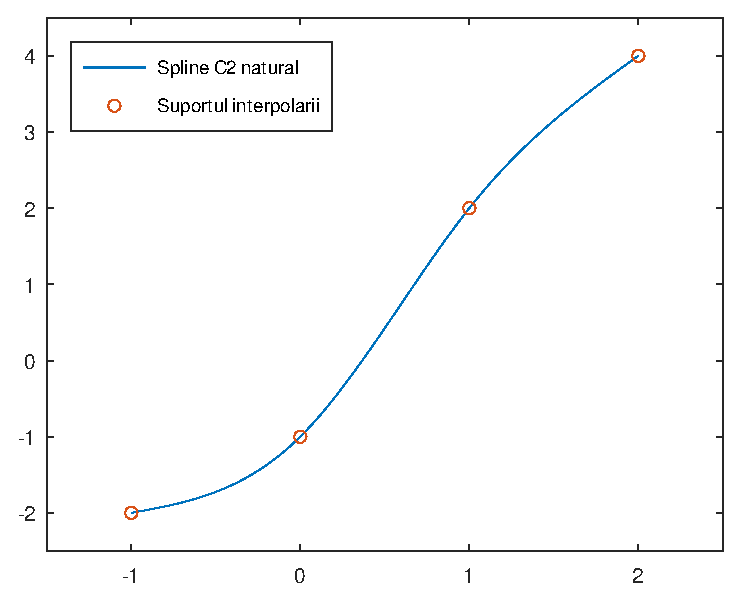
\includegraphics[width=0.45\textwidth]{spline_c2_nat_ex}\hspace{0.5cm}
    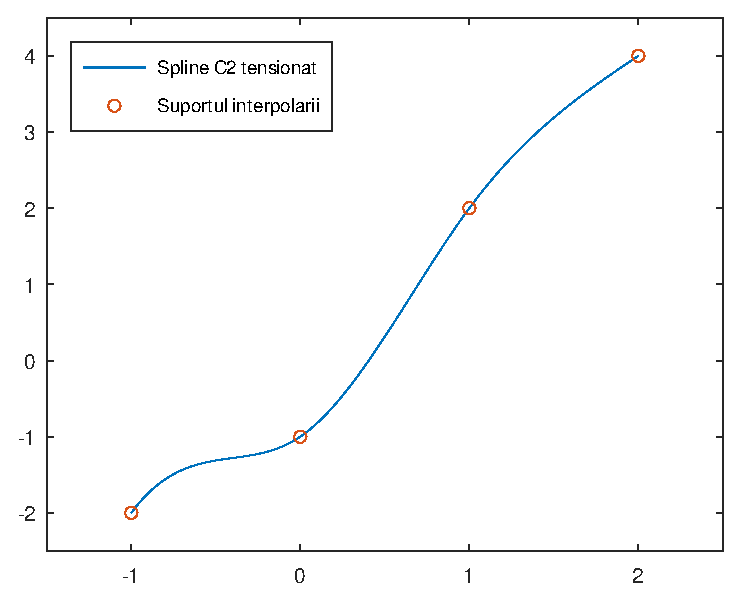
\includegraphics[width=0.45\textwidth]{spline_c2_ten_ex}
\end{center}

\subsection{Concluzii}
\tab
$\oplus$ Dispare fenomenul de oscilatie (la fel ca la $C^1$).\\

$\oplus$ Se impun conditii de racordare mai puternice decat la $C^1$, astfel spline-ul va reda mai bine realitatea.\\

$\oplus$ Este necesar sa se cunoasca valorile derivatei I in capetele suportului de interpolare (\textbf{doar} pentru spline-urile tensionate). \\

\section{Curbe B\'ezier}
\label{sec:bezier}

\subsection{Notiuni generale}

\begin{minipage}{0.75\textwidth}
    \tabto{0.5cm} O curba \textit{B\'ezier} este o curba \textit{parametrica} cu importante aplicatii in grafica pe calculator. Primeste ca input niste \textit{puncte in plan} ($P_0, P_1, \dots, P_{n-1}, P_n$):
    
    \begin{itemize}
        \item Punctele $P_0$ si $P_n$ se numesc \textit{puncte de interpolare (anchor points)},\\deoarece curba B\'ezier trece prin ele (incepe in $P_0$ si se termina in $P_1$).
        
        \item Punctele $P_1, \dots, P_{n-1}$ se numesc \textit{puncte de control (handle points)},\\deoarece ele influenteaza path-ul curbei B\'ezier.
    \end{itemize}
\end{minipage}
\begin{minipage}{0.25\textwidth}
    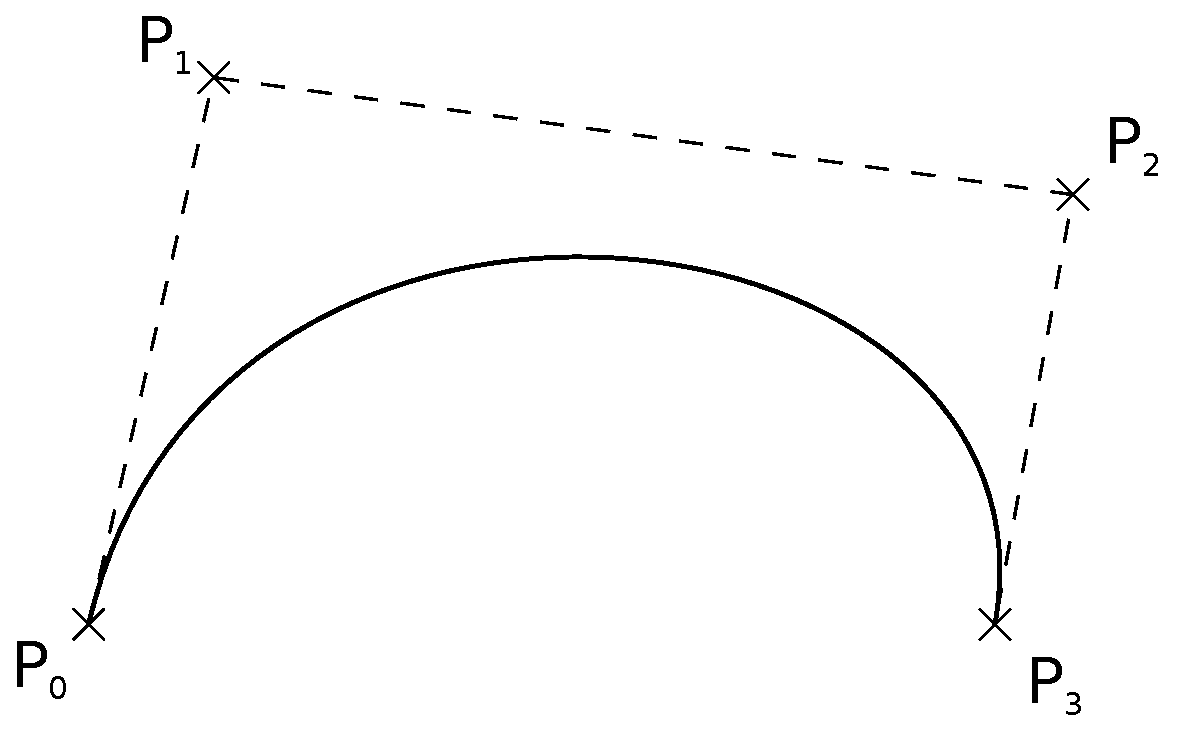
\includegraphics[width=1.5\textwidth]{bezier_ex_n3}
\end{minipage}

La modul general, curba B\'ezier de grad $n$ este definita astfel:
\framebox{$B_n(t) = \sum\limits_{i=0}^{n} P_i \cdot B_{i,n}(t),\; t \in [0, 1]$}, unde:
$\begin{cases}
  P_i\; $sunt punctele de intrare$ \\
  B_{i,n}(t)\; $sunt polinoamele \textit{Bernstein} de grad $n$: $ $\framebox{$B_{i,n}(t) \; \eqdef \; C_n^i \cdot (1-t)^{n-i} \cdot t^i$}$
\end{cases}$

\subsection{Modul de determinare}

\tab Particularizam forma generala a curbei B\'ezier pentru $n=1$, $n=2$ si $n=3$: 
\begin{itemize}
    \item Curba B\'ezier Liniara ($n=1$) \framebox{\href{https://imgur.com/UmXN4T6}{Animatie}} \\
    Este similara cu interpolarea liniara sau parametrizarea segmentului.\\
    $B_1(t) = P_0 \cdot B_{0,1}(t) + P_1 \cdot B_{1,1}(t) \Rightarrow$ $\framebox{$B_1(t) = (1-t) \cdot P_0 + P_1,\; t \in [0, 1]$}$ \\
    
    \item Curba B\'ezier Patratica ($n=2$)
    \framebox{\href{https://imgur.com/kTmmOoN}{Animatie}} \\
    $B_2(t) = P_0 \cdot B_{0,2}(t) + P_1 \cdot B_{1,2}(t) + P_2 \cdot B_{2,2}(t) \Rightarrow$ 
    $\framebox{$B_2(t) = (1-t)^2 \cdot P_0 + 2\cdot t \cdot (1-t) \cdot P_1 + t^2 \cdot P_2,\; t \in [0, 1]$}$ \\
    
    \item Curba B\'ezier Cubica ($n=3$)
    \framebox{\href{https://imgur.com/srTzz7J}{Animatie}} \\
    $B_3(t) = P_0 \cdot B_{0,3}(t) + P_1 \cdot B_{1,3}(t) + P_2 \cdot B_{2,3}(t) + P_3 \cdot B_{3,3}(t) \\ \Rightarrow$ 
    $\framebox{$B_3(t) = (1-t)^3 \cdot P_0 + 3\cdot t \cdot (1-t)^2 \cdot P_1 + 3 \cdot t^2 \cdot (1-t) \cdot P_2 + t^3 \cdot P_3,\; t \in [0, 1]$}$ \\
    
\end{itemize}

\begin{minipage}{0.75\textwidth}
    \tabto{0.5cm} Pentru explicatii suplimentare referitoare la modul de constructie al curbelor B\'ezier:\framebox[0.3cm][r]{\footnotemark}
    
    \tabto{0.5cm} Orice curba B\'ezier este continuta complet in poligonul convex definit de punctele $P_0, P_1, \dots, P_n$ (are proprietatea de \textit{convex hull})
\end{minipage}
\begin{minipage}{0.25\textwidth}
    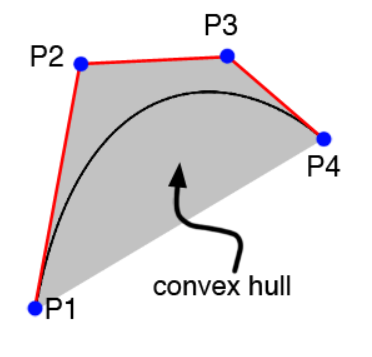
\includegraphics[width=0.75\textwidth]{convex_hull}
\end{minipage}

\footnotetext{\framebox[6.55cm]{\url{https://www.youtube.com/watch?v=pnYccz1Ha34}}}

In mod uzual, se folosesc curbe B\'ezier \textit{cubice} determinate de 4 puncte $P_0, P_1, P_2$, $P_3$, avand forma parametrica determinata anterior:

$B_3(t) = (1-t)^3 \cdot P_0 + 3\cdot t \cdot (1-t)^2 \cdot P_1 + 3 \cdot t^2 \cdot (1-t) \cdot P_2 + t^3 \cdot P_3$, $t \in [0, 1]$

$\Longrightarrow$
\framebox{
$B_3(t) =$
$\begin{bmatrix}
    t^3 & t^2 & t & 1 \\
\end{bmatrix} \cdot $
$\begin{bmatrix}[r]
    -1 & 3 & -3 & 1 \\
    3 & -6 & 3 & 0 \\
    -3 & 3 & 0 & 0 \\
    1 & 0 & 0 & 0 \\
\end{bmatrix} \cdot $
$\begin{bmatrix}
    P_0 \\
    P_1 \\
    P_2 \\
    P_3 \\
\end{bmatrix}$}
$,\;t \in [0, 1]$\\

Observati cum se schimba path-ul curbei B\'ezier odata cu modificarea pozitiei punctelor de control \framebox[0.4cm][r]{\footnotemark}.
\footnotetext{\framebox[6.725cm]{\url{https://www.desmos.com/calculator/gptceium9j}}}


Observatie: Pentru puncte in spatiu, notiunea de curba B\'ezier se extinde la \textit{suprafata B\'ezier} \framebox[0.4cm][r]{\footnotemark}.
\footnotetext{\framebox[3.5cm]{\url{https://bit.ly/2W60onD}}}

Asadar, pentru a determina curba B\'ezier de grad $n$, ne folosim de polinoamele Bernstein de grad $n$.

Asa cum am vazut, polinoamele Bernstein se pot calcula si \textit{recurent}.

Pentru a facilita calculul computerizat al curbei B\'ezier, introducem algoritmul \textbf{De Casteljau}.

\section{Algoritmul De Casteljau}
\label{sec:casteljau}

\subsection{Notiuni generale}
\tab Intr-o abordare directa, calcularea unui punct aflat pe o curba B\'ezier se obtine folosind ecuatia parametrica $B_n(t) = \sum\limits_{i=0}^{n} P_i \cdot B_{i,n}(t),\; t \in [0, 1]$.

Aceasta metoda este ineficienta, deoarece este instabila numeric (numerele mici ridicate la puteri mari, genereaza erori).

Algoritmul De Casteljau este o metoda recursiva de calcul a polinoamelor Bernstein folosite in determinarea curbelor B\'ezier. \\

\begin{itemize}
    \item Date de \textit{intrare}: Punctele $P_0, P_1, \dots, P_n$.
    
    \item Se foloseste relatia de \textit{recurenta}:

        \tabto{1cm} $P_i^{(0)} = P_i,\; i = 0 : n$
        
        \tabto{1cm} for $j = 1 : n$
        
        \tabto{1.5cm} for $i = 0 : n-j$
        
        \tabto{2cm} $P_i^{(j)} = P_i^{(j-1)} \cdot (1-t) + P_{i+1}^{(j-1)} \cdot t$
        
    \item Date de \textit{iesire}: $P_0^{(n)}$
\end{itemize}

Observatie: $P_i^{(j)}$ reprezinta punctul $P_i$ la pasul $j$. \\\\


Fie $P_i^{(0)}$ si $P_{i+1}^{(0)}$ doua puncte succesive si $P_i^{(1)}$ un punct care imparte segmentul $P_i^{(0)}P_{i+1}^{(0)}$ in raportul $\frac{t}{1-t}$. Atunci, $P_i^{(1)}$ este o combinatie liniara intre punctele $P_i^{(0)}$ si $P_{i+1}^{(0)}$, adica: $P_i^{(1)} = (1-t) \cdot P_i^{(0)} + t \cdot P_{i+1}^{(0)}$

Se formeaza in acest fel poligonul $P_0^{(1)}, P_1^{(1)}, \dots, P_{n-1}^{(1)}$. Se aplica relatia de recurenta noului poligon, obtinandu-se poligonul $P_0^{(2)}, P_1^{(2)}, \dots, P_{n-2}^{(2)}$. Repetand procesul de $n$ ori, se obtine un singur punct $P_0^{(n)}$. Acest punct obtinut se afla pe curba B\'ezier. \\
 

Pentru a intelege mai bine cum functioneaza algoritmul, vom particulariza $n=3$, adica vom construi o curba B\'ezier de grad $3$. Ideea din spatele algoritmului este prezentata grafic aici \framebox[0.4cm][r]{\footnotemark}.

\footnotetext{\framebox[6.6cm]{\url{https://www.youtube.com/watch?v=YATikPP2q70}}}


Pentru $n=3$, procesul de obtinere al punctului $P_1^{(3)}(x)$, este prezentat mai jos (indexarea din exemplu este facuta de la $1$):

\begin{center}
\begin{tabular}{ccccccc}
	$P_{1}^{(0)}(x) \equiv P_1$ & {} & {} \\
	{} & $\searrow $  & {}  & {}\\
	{} & {} &  $P_{1}^{(1)}(x) \equiv P_{12}$ & {}\\
	{} & $\nearrow $ & {}  &  $\searrow $\\
	$P_{2}^{(0)}(x) \equiv P_2$ & {} & {} & {} & $P_{1}^{(2)}(x) \equiv P_{1223}$\\
	{} & $\searrow $  & {} &  $\nearrow $ & {} & $\searrow $\\
	{} & {} &  $P_{2}^{(1)}(x) \equiv P_{23}$ & {} & {} & {} & $P_{1}^{(3)}(x) \equiv P$\\
	{} & $\nearrow $  & {} & $\searrow $ & {} & $\nearrow$\\
	$P_{3}^{(0)}(x) \equiv P_3$ & {}  & {}  & {} & $P_{2}^{(2)}(x) \equiv P_{2334}$\\
	{} & $\searrow $  &{} &  $\nearrow $\\
	{} & {} &  $P_{3}^{(1)}(x) \equiv P_{34}$ & {}\\
	{} & $\nearrow $  & {}  \\
	$P_{4}^{(0)}(x) \equiv P_4$ & {}  & {} & {} \\
\end{tabular}
\end{center}


\begin{minipage}{0.2\textwidth}
    \framebox{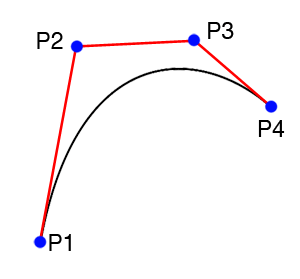
\includegraphics[width=1\textwidth]{decasteljau_0}}
\end{minipage}\;\;\;
{\LARGE{$\rightarrow$}}
\begin{minipage}{0.2\textwidth}
    \framebox{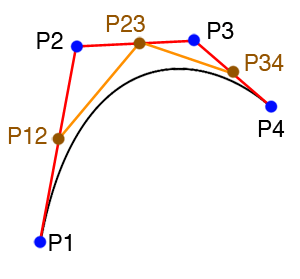
\includegraphics[width=1\textwidth]{decasteljau_1}}
\end{minipage}\;\;
{\LARGE{$\rightarrow$}}
\begin{minipage}{0.2\textwidth}
    \framebox{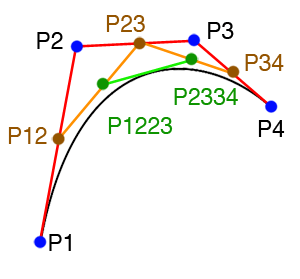
\includegraphics[width=1\textwidth]{decasteljau_2}}
\end{minipage}\;\;
{\LARGE{$\rightarrow$}}
\begin{minipage}{0.2\textwidth}
    \framebox{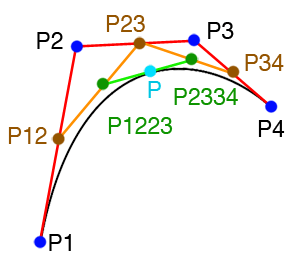
\includegraphics[width=1\textwidth]{decasteljau_3}}
\end{minipage}\\


\subsection{Concluzii}
\tab
$\oplus$ Algoritm stabil numeric.\\

$\ominus$ Mai lent decat abordarea directa (non-recursiva).\\


\section{Probleme Propuse}
\label{sec:probleme}

%New colors defined below
\definecolor{codegreen}{rgb}{0,0.6,0}
\definecolor{codegray}{rgb}{0.5,0.5,0.5}
\definecolor{codepurple}{rgb}{0.58,0,0.82}
\definecolor{backcolour}{rgb}{0.95,0.95,0.92}

%Code listing style named "mystyle"
\lstdefinestyle{mystyle}{
  backgroundcolor=\color{backcolour},   commentstyle=\color{codegreen},
  keywordstyle=\color{magenta},
  numberstyle=\tiny\color{codegray},
  stringstyle=\color{codepurple},
  basicstyle=\ttfamily\footnotesize,
  breakatwhitespace=false,         
  breaklines=true,                 
  captionpos=b,                    
  keepspaces=true,                 
  numbers=left,                    
  numbersep=5pt,                  
  showspaces=false,                
  showstringspaces=false,
  showtabs=false,                  
  tabsize=2
}

%"mystyle" code listing set
\lstset{style=mystyle}

\subsection{Problema 1}
\tab Scrieti un program Octave care interpoleaza un set de date, folosind interpolarea \textbf{Vandermonde}.\\
\tabto{0.5cm} Descarca scriptul:
\href{https://github.com/Iulian277/Interpolation/blob/main/Vandermonde/vandermonde.m}{
\includegraphics[scale=0.35]{download_button}}
\lstinputlisting[language=Octave]{src/vandermonde.m}

Pentru testarea programului, puteti folosi urmatoarea functie:\\
\tabto{0.5cm} Descarca scriptul:
\href{https://github.com/Iulian277/Interpolation/blob/main/Vandermonde/test_vandermonde.m}{
\includegraphics[scale=0.35]{download_button}}
\lstinputlisting[language=Octave]{src/test_vandermonde.m}

Pentru verificare, puteti compara rezultatul vostru cu graficul de aici: \href{https://github.com/Iulian277/Interpolation/blob/main/Vandermonde/vandermonde_res.svg}{
\includegraphics[scale=0.35]{download_button}}

Extra: Puteti rezolva problema si pe hartie si astfel determinati coeficientii polinomului de interpolare.\pagebreak


\subsection{Problema 2}
\tab Scrieti un program Octave care interpoleaza un set de date, folosind interpolarea \textbf{Lagrange}.\\
\tabto{0.5cm} Descarca scriptul:
\href{https://github.com/Iulian277/Interpolation/blob/main/Lagrange/lagrange.m}{
\includegraphics[scale=0.35]{download_button}}
\lstinputlisting[language=Octave]{src/lagrange.m}\vspace{0.25cm}

Pentru testarea programului, puteti folosi urmatoarea functie:\\
\tabto{0.5cm} Descarca scriptul:
\href{https://github.com/Iulian277/Interpolation/blob/main/Lagrange/test_lagrange.m}{
\includegraphics[scale=0.35]{download_button}}
\lstinputlisting[language=Octave]{src/test_lagrange.m}

Pentru verificare, puteti compara rezultatul vostru cu graficul de aici: \href{https://github.com/Iulian277/Interpolation/blob/main/Lagrange/lagrange_res.svg}{
\includegraphics[scale=0.35]{download_button}}

Extra: Puteti rezolva problema si pe hartie si astfel determinati coeficientii polinomului de interpolare.\pagebreak


\subsection{Problema 3}
\tab Scrieti un program Octave care interpoleaza un set de date, folosind interpolarea \textbf{Newton}.\\
\tabto{0.5cm} Descarca scriptul:
\href{https://github.com/Iulian277/Interpolation/blob/main/Newton/newton.m}{
\includegraphics[scale=0.35]{download_button}}
\lstinputlisting[language=Octave]{src/newton.m}\vspace{0.25cm}

Pentru testarea programului, puteti folosi urmatoarea functie:\\
\tabto{0.5cm} Descarca scriptul:
\href{https://github.com/Iulian277/Interpolation/blob/main/Newton/test_newton.m}{
\includegraphics[scale=0.35]{download_button}}
\lstinputlisting[language=Octave]{src/test_newton.m}

Pentru verificare, puteti compara rezultatul vostru cu graficul de aici: \href{https://github.com/Iulian277/Interpolation/blob/main/Newton/newton_res.svg}{
\includegraphics[scale=0.35]{download_button}}

Extra: Puteti rezolva problema si pe hartie si astfel determinati coeficientii polinomului de interpolare.\pagebreak


\subsection{Problema 4}
\tab Scrieti un program Octave care interpoleaza un set de date, folosind functii \textbf{Spline} $\mathbf{C^2}$ \textbf{Natural}.\\
\tabto{0.5cm} Descarca scriptul:
\href{https://github.com/Iulian277/Interpolation/blob/main/Spline\%20C2\%20Natural/splineC2_natural.m}{\includegraphics[scale=0.35]{download_button}}
\lstinputlisting[language=Octave]{src/splineC2_natural.m}\vspace{0.25cm}

Pentru testarea programului, puteti folosi urmatoarea functie:\\
\tabto{0.5cm} Descarca scriptul:
\href{https://github.com/Iulian277/Interpolation/blob/main/Spline\%20C2\%20Natural/test_splineC2_natural.m}{\includegraphics[scale=0.35]{download_button}}
\lstinputlisting[language=Octave]{src/test_splineC2_natural.m}

Pentru verificare, puteti compara rezultatul vostru graficul de aici: \href{https://github.com/Iulian277/Interpolation/blob/main/Spline\%20C2\%20Natural/splineC2_res.svg}{\includegraphics[scale=0.35]{download_button}}

Extra: Puteti rezolva problema si pe hartie si astfel determinati coeficientii spline-urilor.


\subsection{Extra}
\tab In incheiere, puteti lectura un material referitor la utilizarea interpolarii intr-o aplicatie din viata reala (\textbf{Heat Transfer}): \href{http://github.com/Iulian277/Interpolation/blob/main/Heat_Transfer_Interpolation.pdf}{\includegraphics[scale=0.4]{document_button}}

\end{document}
